
\newpage

\begin{figure}
  \begin{minipage}[b][10cm][s]{0.45\textwidth}
    \centering
    \vfill
    \begin{tikzpicture}[scale=0.8]
      \begin{axis}[
    xmode=log,
    ymin=0,ymax=20,
    xmin=0.1, xmax=1000000,
    every axis plot/.style={thin},
    xlabel={timeout limit (ms)},
    ylabel={\# solved},
    legend pos=south east
    % table/create on use/cumulative distribution/.style={
    %   create col/expr={\pgfmathaccuma + \thisrow{f(x)}}   
    % }
    ]
    \addplot 
    [mark=triangle*,
    mark size=1.5,
    mark options={solid},
    green] 
    coordinates {(0.088, 1)
(0.182, 2)
(0.233, 3)
(0.942, 4)
(1.622, 5)
(4.020, 6)
(7.439, 7)
(7.733, 8)
(8.229, 9)
(10.629, 10)
(16.624, 11)
(40.292, 12)
(67.440, 13)
(1244.797, 14)
(7858.266, 15)
(1000001.583, 16)
(1000001.852, 17)
(1009212.178, 18)
(1012657.780, 19)
(1012814.040, 20)};

    \addplot 
    [blue,
    mark=*,
    mark size=1.5,
    mark options={solid}]
    coordinates {(0.084, 1)
(0.206, 2)
(0.217, 3)
(0.871, 4)
(1.393, 5)
(4.322, 6)
(7.026, 7)
(7.901, 8)
(7.904, 9)
(10.663, 10)
(18.990, 11)
(50.266, 12)
(96.214, 13)
(1467.636, 14)
(9916.340, 15)
(1000001.971, 16)
(1000002.938, 17)
(1000004.363, 18)
(1000005.402, 19)
(1000011.197, 20)};

    \addplot [brown!60!black,
    mark options={fill=brown!40},
    mark=otimes*,
    mark size=1.5]
    table {(0.087, 1)
(0.236, 2)
(0.311, 3)
(1.152, 4)
(1.786, 5)
(5.762, 6)
(8.968, 7)
(10.301, 8)
(10.566, 9)
(15.086, 10)
(23.403, 11)
(63.558, 12)
(119.651, 13)
(1877.973, 14)
(13098.088, 15)
(1000002.296, 16)
(1000003.170, 17)
(1000007.159, 18)
(1000007.877, 19)
(1000015.365, 20)};

    \addplot 
    [red,
    mark size=1.5,
    mark=square*]
    table {(0.081, 1)
(0.157, 2)
(0.223, 3)
(0.596, 4)
(0.895, 5)
(2.233, 6)
(4.192, 7)
(4.233, 8)
(4.349, 9)
(5.717, 10)
(8.703, 11)
(21.423, 12)
(37.126, 13)
(669.099, 14)
(4203.782, 15)
(1000000.429, 16)
(1000000.554, 17)
(1000000.652, 18)
(1000000.873, 19)
(1000001.178, 20)};
    \legend{Reg,Tup\_mem,Tup\_speed,CT}
  \end{axis}

    \end{tikzpicture}
    \vfill
    \caption{\textbf{Langford 2}.}
    \vspace{\baselineskip}
  \end{minipage}\qquad
  \begin{minipage}[b][10cm][s]{0.45\textwidth}
    \centering
    \vfill
    \begin{tikzpicture}[scale=0.8]
      \begin{axis}[
    xmode=log,
    ymin=0,ymax=16,
    xmin=0.1, xmax=1000000,
    every axis plot/.style={thin},
    xlabel={timeout limit (ms)},
    ylabel={\# solved},
    legend pos=south east
    % table/create on use/cumulative distribution/.style={
    %   create col/expr={\pgfmathaccuma + \thisrow{f(x)}}   
    % }
    ]
    \addplot 
    [mark=triangle*,
    mark size=1.5,
    mark options={solid},
    green] 
    coordinates {(0.101, 1)
(0.159, 2)
(0.385, 3)
(1.631, 4)
(6.760, 5)
(27.796, 6)
(130.974, 7)
(131.594, 8)
(460.229, 9)
(11472.663, 10)
(18145.843, 11)
(53170.447, 12)
(281456.879, 13)
(1000007.563, 14)
(1000007.588, 15)
(1000013.342, 16)};

    \addplot 
    [blue,
    mark=*,
    mark size=1.5,
    mark options={solid}]
    coordinates {(0.076, 1)
(0.129, 2)
(0.375, 3)
(1.684, 4)
(6.892, 5)
(35.105, 6)
(146.741, 7)
(167.561, 8)
(642.014, 9)
(18202.298, 10)
(42684.881, 11)
(82959.726, 12)
(490547.070, 13)
(1000011.196, 14)
(1000016.557, 15)
(1000016.694, 16)};

    \addplot [brown!60!black,
    mark options={fill=brown!40},
    mark=otimes*,
    mark size=1.5]
    table {(0.090, 1)
(0.166, 2)
(0.510, 3)
(2.198, 4)
(8.900, 5)
(37.617, 6)
(192.203, 7)
(218.167, 8)
(737.821, 9)
(20345.581, 10)
(46306.577, 11)
(103637.500, 12)
(597597.517, 13)
(1000020.102, 14)
(1000020.695, 15)
(1000030.283, 16)};

    \addplot 
    [red,
    mark size=1.5,
    mark=square*]
    table {(0.084, 1)
(0.120, 2)
(0.282, 3)
(1.077, 4)
(4.754, 5)
(20.901, 6)
(95.743, 7)
(100.046, 8)
(388.791, 9)
(9911.345, 10)
(20137.299, 11)
(50724.854, 12)
(291121.550, 13)
(1000003.563, 14)
(1000003.963, 15)
(1000006.252, 16)};
    \legend{Reg,Tup\_mem,Tup\_speed,CT}
  \end{axis}

    \end{tikzpicture}
    \vfill
    \caption{\textbf{Langford 3}.}
    \vspace{\baselineskip}
  \end{minipage}\qquad
  \begin{minipage}[b][10cm][s]{0.45\textwidth}
    \centering
    \vfill
    \begin{tikzpicture}[scale=0.8]
      \begin{axis}[
    xmode=log,
    ymin=0,ymax=12,
    xmin=0.1, xmax=1000000,
    every axis plot/.style={thin},
    xlabel={timeout limit (ms)},
    ylabel={\# solved},
    legend pos=south east
    % table/create on use/cumulative distribution/.style={
    %   create col/expr={\pgfmathaccuma + \thisrow{f(x)}}   
    % }
    ]
    \addplot 
    [mark=triangle*,
    mark size=1.5,
    mark options={solid},
    green] 
    coordinates {(0.065, 1)
(0.087, 2)
(0.289, 3)
(1.562, 4)
(8.000, 5)
(30.401, 6)
(117.094, 7)
(357.814, 8)
(1310.778, 9)
(5831.375, 10)
(19230.909, 11)
(73869.663, 12)};

    \addplot 
    [blue,
    mark=*,
    mark size=1.5,
    mark options={solid}]
    coordinates {(0.072, 1)
(0.093, 2)
(0.379, 3)
(1.721, 4)
(8.377, 5)
(37.488, 6)
(134.316, 7)
(429.198, 8)
(2113.861, 9)
(8563.558, 10)
(31016.505, 11)
(145924.031, 12)};

    \addplot [brown!60!black,
    mark options={fill=brown!40},
    mark=otimes*,
    mark size=1.5]
    table {(0.093, 1)
(0.134, 2)
(0.568, 3)
(2.272, 4)
(11.999, 5)
(50.454, 6)
(172.514, 7)
(535.123, 8)
(2747.097, 9)
(10711.675, 10)
(37336.874, 11)
(156639.352, 12)};

    \addplot 
    [red,
    mark size=1.5,
    mark=square*]
    table {(0.058, 1)
(0.079, 2)
(0.316, 3)
(1.151, 4)
(6.377, 5)
(27.735, 6)
(116.006, 7)
(419.905, 8)
(1794.299, 9)
(7302.931, 10)
(24469.596, 11)
(103661.185, 12)};
    \legend{Reg,Tup\_mem,Tup\_speed,CT}
  \end{axis}

    \end{tikzpicture}
    \vfill
    \caption{\textbf{Langford 4}.}
    \vspace{\baselineskip}
  \end{minipage}\qquad
\end{figure}

\newpage

 \begin{figure}

   \begin{minipage}[b][10cm][s]{.45\textwidth}
     \centering
    \vfill
    \begin{tikzpicture}[scale=0.8]
      \begin{tikzpicture}[scale=1.0]
  \begin{axis}[
    xmode=log,
    ymin=0,ymax=10,
    xmin=0.1, xmax=1000000,
    every axis plot/.style={thin},
    xlabel={timeout limit (ms)},
    ylabel={\# solved},
    legend pos=south east
    % table/create on use/cumulative distribution/.style={
    %   create col/expr={\pgfmathaccuma + \thisrow{f(x)}}   
    % }
    ]
    \addplot 
    [mark=triangle*,
    mark size=1.5,
    mark options={solid},
    green] 
    coordinates {(3900.253,1)
(14195.216,2)
(14700.208,3)
(15990.676,4)
(32710.632,5)
(54054.376,6)
(67230.989,7)
(104769.511,8)
(187327.676,9)
(456587.256,10)};

    \addplot 
    [blue,
    mark=*,
    mark size=1.5,
    mark options={solid}]
    coordinates {(1961.268,1)
(5527.580,2)
(6748.165,3)
(8621.466,4)
(21160.445,5)
(36693.509,6)
(40142.354,7)
(57348.198,8)
(64007.558,9)
(232808.620,10)};

    \addplot [brown!60!black,
    mark options={fill=brown!40},
    mark=otimes*,
    mark size=1.5]
    table {(2919.220,1)
(9242.704,2)
(10216.961,3)
(12505.739,4)
(36508.070,5)
(41345.093,6)
(63946.199,7)
(93165.829,8)
(93608.522,9)
(353637.305,10)};

    \addplot 
    [red,
    mark size=1.5,
    mark=square*]
    table {(457.829,1)
(1439.246,2)
(1624.748,3)
(1809.718,4)
(6452.936,5)
(11506.164,6)
(14015.848,7)
(16541.901,8)
(16855.847,9)
(57660.351,10)};
    \legend{Reg,Tup\_mem,Tup\_speed,CT}
  \end{axis}
\end{tikzpicture}

    \end{tikzpicture}    
    \vfill
    \caption{Rands JC2500.}\label{fig:simple2}
    \vspace{\baselineskip}
  \end{minipage}\qquad
  \begin{minipage}[b][10cm][s]{.45\textwidth}
    \centering
    \vfill
    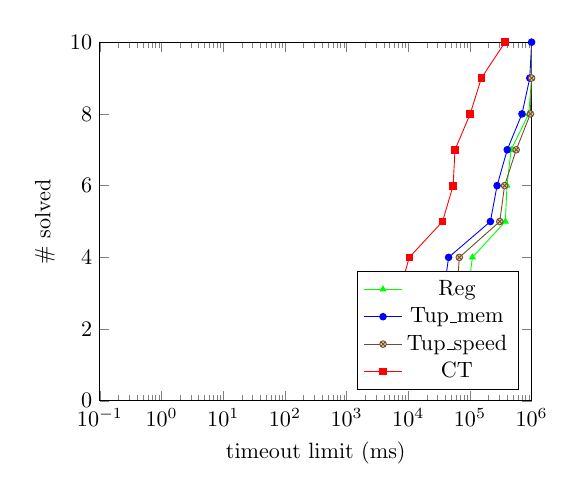
\begin{tikzpicture}[scale=0.8]
      \begin{axis}[
    xmode=log,
    ymin=0,ymax=10,
    xmin=0.1, xmax=1000000,
    every axis plot/.style={thin},
    xlabel={timeout limit (ms)},
    ylabel={\# solved},
    legend pos=south east
    % table/create on use/cumulative distribution/.style={
    %   create col/expr={\pgfmathaccuma + \thisrow{f(x)}}   
    % }
    ]
    \addplot 
    [mark=triangle*,
    mark size=1.5,
    mark options={solid},
    green] 
    coordinates {(31574.208, 1)
(89069.596, 2)
(92409.911, 3)
(109617.692, 4)
(375120.195, 5)
(398745.546, 6)
(464795.600, 7)
(896628.914, 8)
(1000000.519, 9)
(1000001.313, 10)};

    \addplot 
    [blue,
    mark=*,
    mark size=1.5,
    mark options={solid}]
    coordinates {(27237.714, 1)
(35441.131, 2)
(37441.293, 3)
(45077.352, 4)
(214515.372, 5)
(275244.504, 6)
(402643.388, 7)
(697541.797, 8)
(934131.437, 9)
(1000000.647, 10)};

    \addplot [brown!60!black,
    mark options={fill=brown!40},
    mark=otimes*,
    mark size=1.5]
    coordinates {(27847.614, 1)
(43395.528, 2)
(61320.788, 3)
(67245.864, 4)
(304719.299, 5)
(364282.419, 6)
(562899.918, 7)
(955072.437, 8)
(1000000.276, 9)
(1000185.158, 10)};

    \addplot 
    [red,
    mark size=1.5,
    mark=square*]
    coordinates {(4559.768, 1)
(5269.384, 2)
(7089.864, 3)
(10389.645, 4)
(35953.097, 5)
(53378.404, 6)
(57293.505, 7)
(100925.480, 8)
(153336.848, 9)
(371551.862, 10)};
    \legend{Reg,Tup\_mem,Tup\_speed,CT}
  \end{axis}

    \end{tikzpicture}
    \vfill
    \caption{Rands JC5000.}\label{fig:simple2}
    \vspace{\baselineskip}
  \end{minipage}\qquad

  \begin{minipage}[b][10cm][s]{.45\textwidth}
    \centering
    \vfill
    \begin{tikzpicture}[scale=0.8]
      \begin{tikzpicture}[scale=1.0]
  \begin{axis}[
    xmode=log,
    ymin=0,ymax=10,
    xmin=0.1, xmax=1000000,
    every axis plot/.style={thin},
    xlabel={timeout limit (ms)},
    ylabel={\# solved},
    legend pos=south east
    % table/create on use/cumulative distribution/.style={
    %   create col/expr={\pgfmathaccuma + \thisrow{f(x)}}   
    % }
    ]
    \addplot 
    [mark=triangle*,
    mark size=1.5,
    mark options={solid},
    green] 
    coordinates {139268.423 1
140601.911 2
177941.502 3
424666.930 4
1000000.472 5
1000000.888 6
1000001.221 7
1000001.407 8
1000001.457 9
1000003.369 10};

    \addplot 
    [blue,
    mark=*,
    mark size=1.5,
    mark options={solid}]
    coordinates {87932.493 1
117877.394 2
124316.924 3
273988.271 4
850622.333 5
1000000.839 6
1000001.004 7
1000001.005 8
1000001.889 9
1000002.453 10};

    \addplot [brown!60!black,
    mark options={fill=brown!40},
    mark=otimes*,
    mark size=1.5]
    table {122789.372 1
146789.073 2
167882.645 3
363255.524 4
1000000.384 5
1000001.258 6
1000002.593 7
1000002.808 8
1000003.164 9
1000004.253 10};

    \addplot 
    [red,
    mark size=1.5,
    mark=square*]
    table {11372.849 1
16562.793 2
18623.245 3
39394.203 4
121998.328 5
124778.898 6
201796.350 7
436664.869 8
954480.066 9
1000000.181 10};
    \legend{Reg,Tup\_mem,Tup\_speed,CT}
  \end{axis}
\end{tikzpicture}

    \end{tikzpicture}
    \vfill
    \caption{\textbf{Rands JC7500}.}
    \vspace{\baselineskip}
  \end{minipage}\qquad
  \begin{minipage}[b][10cm][s]{.45\textwidth}
    \centering
    \vfill
    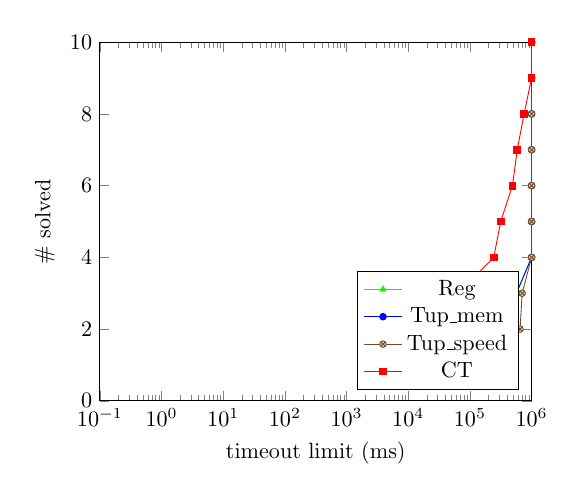
\begin{tikzpicture}[scale=0.8]
      \begin{axis}[
    xmode=log,
    ymin=0,ymax=10,
    xmin=0.1, xmax=1000000,
    every axis plot/.style={thin},
    xlabel={timeout limit (ms)},
    ylabel={\# solved},
    legend pos=south east
    % table/create on use/cumulative distribution/.style={
    %   create col/expr={\pgfmathaccuma + \thisrow{f(x)}}   
    % }
    ]
    \addplot 
    [mark=triangle*,
    mark size=1.5,
    mark options={solid},
    green] 
    coordinates {(332745.543, 1)
(523863.709, 2)
(569686.426, 3)
(1000000.172, 4)
(1000000.554, 5)
(1000000.920, 6)
(1000001.037, 7)
(1000001.490, 8)
(1000002.276, 9)
(1000003.312, 10)};

    \addplot 
    [blue,
    mark=*,
    mark size=1.5,
    mark options={solid}]
    coordinates {(226152.398, 1)
(491387.804, 2)
(566477.841, 3)
(1000000.822, 4)
(1000001.468, 5)
(1000001.597, 6)
(1000001.921, 7)
(1000002.047, 8)
(1000002.465, 9)
(1000003.238, 10)};

    \addplot [brown!60!black,
    mark options={fill=brown!40},
    mark=otimes*,
    mark size=1.5]
    coordinates {(294414.233, 1)
(649951.472, 2)
(702865.808, 3)
(1000000.517, 4)
(1000000.699, 5)
(1000000.802, 6)
(1000001.295, 7)
(1000001.350, 8)
(1000001.480, 9)
(1000001.637, 10)};

    \addplot 
    [red,
    mark size=1.5,
    mark=square*]
    coordinates {(25774.100, 1)
(57124.920, 2)
(64359.631, 3)
(243389.037, 4)
(315549.601, 5)
(489096.976, 6)
(584890.320, 7)
(755476.499, 8)
(1000000.186, 9)
(1000000.225, 10)};
    \legend{Reg,Tup\_mem,Tup\_speed,CT}
  \end{axis}

    \end{tikzpicture}
    \vfill
    \caption{\textbf{Rands JC10000}.}
    \vspace{\baselineskip}
  \end{minipage}\qquad

\end{figure}

\newpage

\begin{figure}
  
  \begin{minipage}[b][10cm][s]{0.45\textwidth}
    \centering
    \vfill
    \begin{tikzpicture}[scale=0.8]
      \begin{tikzpicture}[scale=1.0]
  \begin{axis}[
    xmode=log,
    ymin=0,ymax=23,
    xmin=0.1, xmax=1000000,
    every axis plot/.style={thin},
    xlabel={timeout limit (ms)},
    ylabel={\# solved},
    legend pos=south east
    % table/create on use/cumulative distribution/.style={
    %   create col/expr={\pgfmathaccuma + \thisrow{f(x)}}   
    % }
    ]
    \addplot 
    [mark=triangle*,
    mark size=1.5,
    mark options={solid},
    green] 
    coordinates {0.390 1
0.407 2
0.408 3
0.429 4
0.449 5
0.454 6
0.474 7
0.490 8
0.492 9
0.495 10
0.498 11
0.502 12
0.513 13
0.530 14
0.554 15
0.757 16
0.759 17
1.097 18
1.538 19
1.686 20
1.847 21
4.286 22
5.242 23};

    \addplot 
    [blue,
    mark=*,
    mark size=1.5,
    mark options={solid}]
    coordinates {0.431 1
0.706 2
0.742 3
0.771 4
1.021 5
1.885 6
1.911 7
2.208 8
3.074 9
3.167 10
4.797 11
11.430 12
19.852 13
62.120 14
72.766 15
90.320 16
191.654 17
227.574 18
297.702 19
497.460 20
2463.091 21
4400.894 22
7429.957 23};

    \addplot [brown!60!black,
    mark options={fill=brown!40},
    mark=otimes*,
    mark size=1.5]
    table {0.550 1
0.766 2
0.908 3
0.977 4
1.486 5
2.681 6
2.965 7
3.453 8
4.528 9
4.746 10
7.309 11
17.587 12
30.902 13
90.208 14
106.065 15
137.677 16
291.910 17
340.514 18
456.452 19
743.107 20
3772.207 21
6539.383 22
11517.655 23};

    \addplot 
    [red,
    mark size=1.5,
    mark=square*]
    table {0.439 1
0.618 2
0.698 3
0.735 4
1.093 5
1.910 6
2.099 7
2.368 8
2.794 9
3.010 10
4.795 11
11.303 12
19.709 13
53.169 14
61.288 15
66.296 16
156.013 17
182.439 18
253.668 19
338.968 20
1947.380 21
2773.622 22
4557.056 23};
    \legend{Reg,Tup\_mem,Tup\_speed,CT}
  \end{axis}
\end{tikzpicture}

    \end{tikzpicture}
    \vfill
    \caption{\textbf{AIM-50}.}
    \vspace{\baselineskip}
  \end{minipage}\qquad
  \begin{minipage}[b][10cm][s]{0.45\textwidth}
    \centering
    \vfill
    \begin{tikzpicture}[scale=0.8]
      \begin{axis}[
    xmode=log,
    ymin=0,ymax=23,
    xmin=0.1, xmax=1000000,
    every axis plot/.style={thin},
    xlabel={timeout limit (ms)},
    ylabel={\# solved},
    legend pos=south east
    % table/create on use/cumulative distribution/.style={
    %   create col/expr={\pgfmathaccuma + \thisrow{f(x)}}   
    % }
    ]
    \addplot 
    [mark=triangle*,
    mark size=1.5,
    mark options={solid},
    green] 
    coordinates {(0.823, 1)
(0.832, 2)
(0.857, 3)
(0.867, 4)
(0.885, 5)
(0.918, 6)
(0.939, 7)
(0.953, 8)
(0.974, 9)
(0.981, 10)
(0.987, 11)
(0.988, 12)
(1.008, 13)
(1.061, 14)
(1.135, 15)
(1.205, 16)
(2.753, 17)
(3.647, 18)
(24.877, 19)
(24.886, 20)
(35.599, 21)
(42.011, 22)
(48.965, 23)};

    \addplot 
    [blue,
    mark=*,
    mark size=1.5,
    mark options={solid}]
    coordinates {(3.586, 1)
(3.671, 2)
(6.004, 3)
(9.450, 4)
(15.887, 5)
(52.426, 6)
(80.095, 7)
(171.902, 8)
(4436.194, 9)
(41949.006, 10)
(100934.221, 11)
(147492.566, 12)
(556004.535, 13)
(1000000.165, 14)
(1000000.167, 15)
(1000000.174, 16)
(1000000.174, 17)
(1000000.176, 18)
(1000000.179, 19)
(1000000.202, 20)
(1000000.260, 21)
(1000000.266, 22)
(1000000.286, 23)};

    \addplot [brown!60!black,
    mark options={fill=brown!40},
    mark=otimes*,
    mark size=1.5]
    table {(5.211, 1)
(5.793, 2)
(9.033, 3)
(13.782, 4)
(24.369, 5)
(77.669, 6)
(120.860, 7)
(258.984, 8)
(6933.488, 9)
(65101.206, 10)
(165079.465, 11)
(242773.103, 12)
(877436.255, 13)
(1000000.113, 14)
(1000000.118, 15)
(1000000.123, 16)
(1000000.132, 17)
(1000000.154, 18)
(1000000.165, 19)
(1000000.189, 20)
(1000000.191, 21)
(1000000.196, 22)
(1000000.259, 23)};

    \addplot 
    [red,
    mark size=1.5,
    mark=square*]
    table {(3.886, 1)
(4.643, 2)
(6.772, 3)
(11.080, 4)
(17.750, 5)
(62.656, 6)
(87.179, 7)
(187.117, 8)
(4632.128, 9)
(36310.893, 10)
(96431.551, 11)
(140762.037, 12)
(452408.039, 13)
(1000000.102, 14)
(1000000.115, 15)
(1000000.118, 16)
(1000000.134, 17)
(1000000.137, 18)
(1000000.157, 19)
(1000000.200, 20)
(1000000.202, 21)
(1000000.221, 22)
(1000000.239, 23)};
    \legend{Reg,Tup\_mem,Tup\_speed,CT}
  \end{axis}

    \end{tikzpicture}
    \vfill
    \caption{\textbf{AIM-100}.}
    \vspace{\baselineskip}
  \end{minipage}\qquad
  \begin{minipage}[b][10cm][s]{0.45\textwidth}
    \centering
    \vfill
    \begin{tikzpicture}[scale=0.8]
      \begin{axis}[
    xmode=log,
    ymin=0,ymax=22,
    xmin=0.1, xmax=1000000,
    every axis plot/.style={thin},
    xlabel={timeout limit (ms)},
    ylabel={\# solved},
    legend pos=south east
    % table/create on use/cumulative distribution/.style={
    %   create col/expr={\pgfmathaccuma + \thisrow{f(x)}}   
    % }
    ]
    \addplot 
    [mark=triangle*,
    mark size=1.5,
    mark options={solid},
    green] 
    coordinates {(2.092, 1)
(2.153, 2)
(2.207, 3)
(2.224, 4)
(2.353, 5)
(2.410, 6)
(2.444, 7)
(2.462, 8)
(2.486, 9)
(2.626, 10)
(2.638, 11)
(4.751, 12)
(7.714, 13)
(12.349, 14)
(459.348, 15)
(786.654, 16)
(1926.845, 17)
(7178.726, 18)
(13920.549, 19)
(63961.995, 20)
(83629.587, 21)
(215920.851, 22)};

    \addplot 
    [blue,
    mark=*,
    mark size=1.5,
    mark options={solid}]
    coordinates {(92.762, 1)
(214.140, 2)
(5059.466, 3)
(9347.039, 4)
(1000000.212, 5)
(1000000.214, 6)
(1000000.230, 7)
(1000000.234, 8)
(1000000.236, 9)
(1000000.243, 10)
(1000000.247, 11)
(1000000.332, 12)
(1000000.348, 13)
(1000000.356, 14)
(1000000.384, 15)
(1000000.413, 16)
(1000000.580, 17)
(1001526.960, 18)
(1013587.491, 19)
(1015726.858, 20)
(1021700.000, 21)
(1026780.972, 22)};

    \addplot [brown!60!black,
    mark options={fill=brown!40},
    mark=otimes*,
    mark size=1.5]
    table {(144.623, 1)
(333.321, 2)
(9960.406, 3)
(14839.411, 4)
(1000000.132, 5)
(1000000.132, 6)
(1000000.138, 7)
(1000000.154, 8)
(1000000.156, 9)
(1000000.161, 10)
(1000000.176, 11)
(1000000.201, 12)
(1000000.233, 13)
(1000000.233, 14)
(1000000.264, 15)
(1000000.302, 16)
(1000000.338, 17)
(1000000.401, 18)
(1000000.462, 19)
(1000000.559, 20)
(1000201.313, 21)
(1030367.681, 22)};

    \addplot 
    [red,
    mark size=1.5,
    mark=square*]
    table {(120.173, 1)
(264.364, 2)
(6492.284, 3)
(12332.389, 4)
(1000000.117, 5)
(1000000.130, 6)
(1000000.138, 7)
(1000000.141, 8)
(1000000.144, 9)
(1000000.148, 10)
(1000000.157, 11)
(1000000.179, 12)
(1000000.199, 13)
(1000000.223, 14)
(1000000.258, 15)
(1000000.312, 16)
(1000000.349, 17)
(1000000.387, 18)
(1000000.408, 19)
(1019145.714, 20)
(1021004.571, 21)
(1051023.598, 22)};
    \legend{Reg,Tup\_mem,Tup\_speed,CT}
  \end{axis}

    \end{tikzpicture}
    \vfill
    \caption{\textbf{AIM-200}.}
    \vspace{\baselineskip}
  \end{minipage}\qquad
\end{figure}

\newpage

\begin{figure}
  \begin{minipage}[b][10cm][s]{0.45\textwidth}
    \centering
    \vfill
    \begin{tikzpicture}[scale=0.8]
      \begin{tikzpicture}[scale=1.0]
  \begin{axis}[
    xmode=log,
    ymin=0,ymax=50,
    xmin=0.1, xmax=1000000,
    every axis plot/.style={thin},
    xlabel={timeout limit (ms)},
    ylabel={\# solved},
    legend pos=south east
    % table/create on use/cumulative distribution/.style={
    %   create col/expr={\pgfmathaccuma + \thisrow{f(x)}}   
    % }
    ]
    \addplot 
    [mark=triangle*,
    mark size=1.5,
    mark options={solid},
    green] 
    coordinates {21539.047 1
23631.895 2
23716.403 3
24241.194 4
24452.383 5
24702.581 6
24727.049 7
24735.421 8
24762.823 9
25381.219 10
25446.865 11
25447.244 12
25663.048 13
25681.411 14
25705.552 15
25921.922 16
26000.936 17
26206.810 18
26236.781 19
26242.879 20
26255.926 21
26263.647 22
26276.749 23
26572.969 24
26580.275 25
26658.352 26
26798.498 27
27134.428 28
27340.416 29
27401.714 30
27486.019 31
27561.142 32
27728.713 33
27922.916 34
28054.949 35
28057.644 36
28193.151 37
28328.067 38
28495.760 39
28577.913 40
28589.075 41
28945.618 42
29006.507 43
29341.039 44
29520.154 45
29560.978 46
29585.618 47
29688.054 48
29934.812 49
30055.889 50};

    \addplot 
    [blue,
    mark=*,
    mark size=1.5,
    mark options={solid}]
    coordinates {7672.186 1
7964.072 2
7988.188 3
8311.150 4
8326.644 5
8405.755 6
8413.912 7
8433.367 8
8543.205 9
8852.685 10
8991.001 11
9027.728 12
9120.668 13
9300.145 14
9307.344 15
9334.373 16
9427.760 17
9445.763 18
9469.390 19
9514.190 20
9600.928 21
9650.273 22
9746.749 23
9808.637 24
9817.477 25
9908.257 26
9966.772 27
9974.917 28
10107.698 29
10130.344 30
10214.500 31
10354.798 32
10411.441 33
10412.120 34
10566.980 35
10629.555 36
10690.029 37
10750.761 38
10771.949 39
10783.994 40
10796.075 41
10819.530 42
10910.396 43
10935.039 44
11189.948 45
11409.743 46
11725.089 47
11914.318 48
12087.322 49
12551.558 50};

    \addplot [brown!60!black,
    mark options={fill=brown!40},
    mark=otimes*,
    mark size=1.5]
    table {11083.294 1
11942.343 2
12057.186 3
12065.914 4
12165.546 5
12230.996 6
12353.178 7
12499.801 8
12539.423 9
12659.462 10
12724.767 11
12772.533 12
13125.773 13
13328.450 14
13638.694 15
13680.520 16
13726.853 17
13788.117 18
13799.316 19
13929.021 20
13937.426 21
14037.418 22
14066.707 23
14101.725 24
14130.306 25
14152.192 26
14478.238 27
14540.951 28
14544.138 29
14609.419 30
14697.861 31
14702.186 32
14899.661 33
15027.878 34
15089.663 35
15146.606 36
15213.444 37
15229.658 38
15372.915 39
15428.330 40
15796.160 41
15805.142 42
15904.232 43
16049.472 44
16141.290 45
16151.591 46
16160.955 47
16942.804 48
17001.615 49
17047.240 50};

    \addplot 
    [red,
    mark size=1.5,
    mark=square*]
    table {2427.974 1
2699.046 2
2717.750 3
2743.960 4
2797.776 5
2816.502 6
2841.334 7
2900.942 8
2904.804 9
2908.160 10
2910.491 11
2933.117 12
2933.400 13
2967.383 14
2989.519 15
3003.038 16
3029.964 17
3063.311 18
3093.973 19
3141.933 20
3150.100 21
3186.832 22
3220.475 23
3234.416 24
3239.493 25
3269.265 26
3293.108 27
3353.966 28
3379.302 29
3394.468 30
3439.955 31
3458.748 32
3527.174 33
3528.582 34
3540.231 35
3558.883 36
3570.218 37
3574.549 38
3610.825 39
3624.569 40
3627.753 41
3673.298 42
3729.990 43
3743.274 44
3779.422 45
3788.515 46
3859.838 47
3898.223 48
3979.624 49
4133.050 50};
    \legend{Reg,Tup\_mem,Tup\_speed,CT}
  \end{axis}
\end{tikzpicture}

    \end{tikzpicture}
    \vfill
    \caption{\textbf{A5}.}
    \vspace{\baselineskip}
  \end{minipage}\qquad

  \begin{minipage}[b][10cm][s]{0.45\textwidth}
    \centering
    \vfill
    \begin{tikzpicture}[scale=0.8]
      \begin{tikzpicture}[scale=1.0]
  \begin{axis}[
    xmode=log,
    ymin=0,ymax=23,
    xmin=0.1, xmax=1000000,
    every axis plot/.style={thin},
    xlabel={timeout limit (ms)},
    ylabel={\# solved},
    legend pos=south east
    % table/create on use/cumulative distribution/.style={
    %   create col/expr={\pgfmathaccuma + \thisrow{f(x)}}   
    % }
    ]
    \addplot 
    [mark=triangle*,
    mark size=1.5,
    mark options={solid},
    green] 
    coordinates {727435.433 1
1000001.373 2
1000005.483 3
1000006.809 4
1000008.096 5
1000009.635 6
1000010.074 7
1000011.271 8
1000012.432 9
1000012.672 10
1000015.905 11
1000017.026 12
1000022.231 13
1000029.449 14
1000030.270 15
1000031.062 16
1000036.397 17
1000036.748 18
1000039.103 19
1000043.823 20
1000044.070 21
1000052.767 22
1000080.677 23};

    \addplot 
    [blue,
    mark=*,
    mark size=1.5,
    mark options={solid}]
    coordinates {224520.942 1
311434.541 2
518531.192 3
563843.176 4
816767.503 5
1000001.025 6
1000001.573 7
1000003.413 8
1000003.543 9
1000003.636 10
1000004.219 11
1000005.825 12
1000006.947 13
1000008.010 14
1000009.980 15
1000012.435 16
1000015.261 17
1000015.833 18
1000017.025 19
1000023.640 20
1000029.233 21
1000041.787 22
1000054.453 23};

    \addplot [brown!60!black,
    mark options={fill=brown!40},
    mark=otimes*,
    mark size=1.5]
    table {316710.534 1
410461.377 2
648720.274 3
713048.102 4
1000002.616 5
1000004.304 6
1000005.477 7
1000005.720 8
1000009.313 9
1000010.227 10
1000014.478 11
1000014.751 12
1000020.934 13
1000021.694 14
1000022.834 15
1000022.849 16
1000028.045 17
1000028.187 18
1000031.847 19
1000032.588 20
1000032.896 21
1000044.704 22
1000046.876 23};

    \addplot 
    [red,
    mark size=1.5,
    mark=square*]
    table {20486.588 1
58503.164 2
61130.226 3
77146.092 4
94763.488 5
153385.993 6
226208.408 7
402373.676 8
417665.968 9
446212.851 10
455410.096 11
600725.556 12
1000000.185 13
1000000.197 14
1000000.502 15
1000000.985 16
1000001.080 17
1000001.500 18
1000001.515 19
1000001.657 20
1000002.297 21
1000002.778 22
1000003.801 23};
    \legend{Reg,Tup\_mem,Tup\_speed,CT}
  \end{axis}
\end{tikzpicture}

    \end{tikzpicture}
    \vfill
    \caption{\textbf{A10}.}
    \vspace{\baselineskip}
  \end{minipage}\qquad
\end{figure}

\newpage

\begin{figure}
  \begin{minipage}[b][10cm][s]{0.45\textwidth}
    \centering
    \vfill
    \begin{tikzpicture}[scale=0.8]
      \begin{tikzpicture}[scale=1.0]
  \begin{axis}[
    xmode=log,
    ymin=0,ymax=65,
    xmin=0.1, xmax=1000000,
    every axis plot/.style={thin},
    xlabel={timeout limit (ms)},
    ylabel={\# solved},
    legend pos=south east
    % table/create on use/cumulative distribution/.style={
    %   create col/expr={\pgfmathaccuma + \thisrow{f(x)}}   
    % }
    ]
    \addplot 
    [mark=triangle*,
    mark size=1.5,
    mark options={solid},
    green] 
    coordinates {0.078 1
0.089 2
0.089 3
0.093 4
0.094 5
0.095 6
0.095 7
0.097 8
0.098 9
0.098 10
0.099 11
0.099 12
0.099 13
0.102 14
0.103 15
0.103 16
0.106 17
0.157 18
0.831 19
1.490 20
1.498 21
1.518 22
1.954 23
3.734 24
3.737 25
4.347 26
9.191 27
10.580 28
19.169 29
22.780 30
26.266 31
81.558 32
102.447 33
104.991 34
131.512 35
332.462 36
352.388 37
618.827 38
788.523 39
790.494 40
1259.350 41
1678.432 42
1862.544 43
2455.933 44
2837.051 45
3271.878 46
4855.913 47
6934.464 48
7463.727 49
8049.052 50
8952.593 51
19737.517 52
23132.443 53
23469.266 54
26002.371 55
29111.360 56
42946.710 57
73225.089 58
74320.226 59
75593.251 60
108672.990 61
122929.922 62
149958.110 63
163565.715 64
261688.209 65};

    \addplot 
    [blue,
    mark=*,
    mark size=1.5,
    mark options={solid}]
    coordinates {0.342 1
0.351 2
0.361 3
0.400 4
0.401 5
0.420 6
0.433 7
0.433 8
0.436 9
0.442 10
0.476 11
0.489 12
0.492 13
0.493 14
0.549 15
0.590 16
0.652 17
0.720 18
0.923 19
1.008 20
1.184 21
1.528 22
1.727 23
2.724 24
3.600 25
7.208 26
7.829 27
8.978 28
12.102 29
17.784 30
33.887 31
40.219 32
55.846 33
61.501 34
164.731 35
184.236 36
360.816 37
429.133 38
484.976 39
586.591 40
794.649 41
932.019 42
1474.042 43
1555.417 44
1890.818 45
3795.101 46
5347.478 47
6026.047 48
7463.682 49
9392.594 50
12105.731 51
25050.002 52
40536.372 53
48045.798 54
61824.891 55
74212.070 56
143995.198 57
243803.619 58
296870.468 59
302900.312 60
322459.873 61
333997.695 62
444619.255 63
457064.862 64
908177.605 65};

    \addplot [brown!60!black,
    mark options={fill=brown!40},
    mark=otimes*,
    mark size=1.5]
    table {0.702 1
0.797 2
0.808 3
0.911 4
0.944 5
0.954 6
0.961 7
1.001 8
1.027 9
1.096 10
1.103 11
1.108 12
1.156 13
1.178 14
1.190 15
1.198 16
1.218 17
1.346 18
1.419 19
1.807 20
2.596 21
3.899 22
4.099 23
5.733 24
5.889 25
9.553 26
10.532 27
11.796 28
28.281 29
29.933 30
49.328 31
75.166 32
103.942 33
120.948 34
278.999 35
367.701 36
427.636 37
574.683 38
660.416 39
802.131 40
1091.373 41
1360.532 42
1932.804 43
2291.232 44
2682.220 45
5395.569 46
7382.573 47
8090.518 48
8788.504 49
12047.370 50
15892.962 51
30283.964 52
52697.241 53
60018.686 54
76459.238 55
87041.593 56
184487.102 57
286328.868 58
338304.442 59
353888.532 60
366508.306 61
398389.231 62
531168.118 63
545050.662 64
1000001.713 65};

    \addplot 
    [red,
    mark size=1.5,
    mark=square*]
    table {0.069 1
0.069 2
0.080 3
0.086 4
0.086 5
0.089 6
0.089 7
0.089 8
0.090 9
0.091 10
0.092 11
0.092 12
0.093 13
0.093 14
0.094 15
0.096 16
0.099 17
0.101 18
0.365 19
0.406 20
0.422 21
0.510 22
0.784 23
1.236 24
1.591 25
1.712 26
1.824 27
2.622 28
5.997 29
6.538 30
7.745 31
17.398 32
24.309 33
26.727 34
33.697 35
63.005 36
63.138 37
77.013 38
147.914 39
162.476 40
176.882 41
296.947 42
330.613 43
459.449 44
472.783 45
804.999 46
1061.529 47
1140.902 48
1254.905 49
1867.303 50
2462.669 51
4400.046 52
8169.387 53
9165.590 54
9457.464 55
9850.643 56
23517.073 57
36089.500 58
38817.645 59
40027.459 60
47404.529 61
50511.047 62
64207.992 63
70129.605 64
130009.590 65};
    \legend{Reg,Tup\_mem,Tup\_speed,CT}
  \end{axis}
\end{tikzpicture}

    \end{tikzpicture}
    \vfill
    \caption{\textbf{Crosswords WorldVG}.}
    \vspace{\baselineskip}
  \end{minipage}\qquad

    \begin{minipage}[b][10cm][s]{0.45\textwidth}
    \centering
    \vfill
    \begin{tikzpicture}[scale=0.8]
      \begin{axis}[
    xmode=log,
    ymin=0,ymax=63,
    xmin=0.1, xmax=1000000,
    every axis plot/.style={thin},
    xlabel={timeout limit (ms)},
    ylabel={\# solved},
    legend pos=south east
    % table/create on use/cumulative distribution/.style={
    %   create col/expr={\pgfmathaccuma + \thisrow{f(x)}}   
    % }
    ]
    \addplot 
    [mark=triangle*,
    mark size=1.5,
    mark options={solid},
    green] 
    coordinates {(0.074, 1)
(0.076, 2)
(0.078, 3)
(0.082, 4)
(0.089, 5)
(0.089, 6)
(0.092, 7)
(0.096, 8)
(0.097, 9)
(0.097, 10)
(0.097, 11)
(0.099, 12)
(0.099, 13)
(0.102, 14)
(0.103, 15)
(0.108, 16)
(0.117, 17)
(0.123, 18)
(0.500, 19)
(0.676, 20)
(0.723, 21)
(0.905, 22)
(1.332, 23)
(1.692, 24)
(1.766, 25)
(1.791, 26)
(5.276, 27)
(16.858, 28)
(17.927, 29)
(30.069, 30)
(35.255, 31)
(41.801, 32)
(52.490, 33)
(75.080, 34)
(96.307, 35)
(130.683, 36)
(131.067, 37)
(225.774, 38)
(274.112, 39)
(379.638, 40)
(550.637, 41)
(909.264, 42)
(1274.166, 43)
(1388.373, 44)
(2525.152, 45)
(2533.498, 46)
(2595.853, 47)
(4030.753, 48)
(4547.362, 49)
(5055.465, 50)
(5791.415, 51)
(10242.753, 52)
(12298.425, 53)
(14360.436, 54)
(14982.830, 55)
(17458.388, 56)
(20992.013, 57)
(29908.599, 58)
(33944.527, 59)
(36060.331, 60)
(55002.467, 61)
(60672.239, 62)
(76112.252, 63)};

    \addplot 
    [blue,
    mark=*,
    mark size=1.5,
    mark options={solid}]
    coordinates {(0.273, 1)
(0.276, 2)
(0.280, 3)
(0.282, 4)
(0.283, 5)
(0.284, 6)
(0.299, 7)
(0.306, 8)
(0.311, 9)
(0.319, 10)
(0.323, 11)
(0.345, 12)
(0.352, 13)
(0.399, 14)
(0.502, 15)
(0.503, 16)
(0.531, 17)
(0.536, 18)
(0.570, 19)
(0.573, 20)
(0.880, 21)
(1.282, 22)
(1.284, 23)
(1.298, 24)
(1.740, 25)
(2.601, 26)
(3.676, 27)
(4.898, 28)
(9.614, 29)
(9.646, 30)
(17.588, 31)
(26.301, 32)
(53.031, 33)
(63.457, 34)
(140.413, 35)
(155.119, 36)
(167.139, 37)
(223.250, 38)
(272.924, 39)
(302.082, 40)
(761.487, 41)
(945.499, 42)
(1346.690, 43)
(1449.372, 44)
(1491.881, 45)
(2704.616, 46)
(3119.614, 47)
(5009.739, 48)
(5632.408, 49)
(7755.518, 50)
(8079.373, 51)
(13953.623, 52)
(17063.131, 53)
(19618.816, 54)
(21960.324, 55)
(24240.394, 56)
(39633.214, 57)
(64699.544, 58)
(71580.728, 59)
(73166.699, 60)
(112247.995, 61)
(121257.043, 62)
(151915.668, 63)};

    \addplot [brown!60!black,
    mark options={fill=brown!40},
    mark=otimes*,
    mark size=1.5]
    table {(0.412, 1)
(0.457, 2)
(0.458, 3)
(0.464, 4)
(0.471, 5)
(0.484, 6)
(0.496, 7)
(0.516, 8)
(0.572, 9)
(0.572, 10)
(0.598, 11)
(0.679, 12)
(0.734, 13)
(0.864, 14)
(1.027, 15)
(1.106, 16)
(1.203, 17)
(1.280, 18)
(1.557, 19)
(1.667, 20)
(2.002, 21)
(2.016, 22)
(2.303, 23)
(2.819, 24)
(2.952, 25)
(2.970, 26)
(5.162, 27)
(5.506, 28)
(18.023, 29)
(19.081, 30)
(39.969, 31)
(56.794, 32)
(100.167, 33)
(128.098, 34)
(172.182, 35)
(249.519, 36)
(259.430, 37)
(286.138, 38)
(488.848, 39)
(568.244, 40)
(1062.970, 41)
(1350.822, 42)
(1626.744, 43)
(1729.003, 44)
(2145.034, 45)
(3496.611, 46)
(3833.896, 47)
(6131.314, 48)
(7395.849, 49)
(9657.251, 50)
(10635.431, 51)
(17957.948, 52)
(19794.735, 53)
(25594.928, 54)
(27375.416, 55)
(30057.643, 56)
(50552.660, 57)
(78826.698, 58)
(88585.449, 59)
(90256.706, 60)
(134279.170, 61)
(143593.547, 62)
(181192.715, 63)};

    \addplot 
    [red,
    mark size=1.5,
    mark=square*]
    table {(0.068, 1)
(0.068, 2)
(0.069, 3)
(0.070, 4)
(0.072, 5)
(0.073, 6)
(0.073, 7)
(0.075, 8)
(0.077, 9)
(0.080, 10)
(0.081, 11)
(0.084, 12)
(0.087, 13)
(0.087, 14)
(0.088, 15)
(0.088, 16)
(0.089, 17)
(0.090, 18)
(0.091, 19)
(0.093, 20)
(0.350, 21)
(0.416, 22)
(0.568, 23)
(0.568, 24)
(0.626, 25)
(0.803, 26)
(1.154, 27)
(1.608, 28)
(4.334, 29)
(4.592, 30)
(9.543, 31)
(14.146, 32)
(20.935, 33)
(24.430, 34)
(31.227, 35)
(39.168, 36)
(59.321, 37)
(71.346, 38)
(116.614, 39)
(120.688, 40)
(172.687, 41)
(207.521, 42)
(217.931, 43)
(266.423, 44)
(477.466, 45)
(566.003, 46)
(683.586, 47)
(1064.142, 48)
(1232.853, 49)
(1672.169, 50)
(1747.561, 51)
(2681.469, 52)
(2811.215, 53)
(4092.535, 54)
(4387.910, 55)
(5269.595, 56)
(8047.345, 57)
(14122.235, 58)
(14686.169, 59)
(14970.167, 60)
(19502.734, 61)
(26550.723, 62)
(32323.306, 63)};
    \legend{Reg,Tup\_mem,Tup\_speed,CT}
  \end{axis}

    \end{tikzpicture}
    \vfill
    \caption{\textbf{Crosswords LexVG}.}
    \vspace{\baselineskip}
  \end{minipage}\qquad
  \begin{minipage}[b][10cm][s]{0.45\textwidth}
    \centering
    \vfill
    \begin{tikzpicture}[scale=0.8]
      \begin{tikzpicture}[scale=1.0]
  \begin{axis}[
    xmode=log,
    ymin=0,ymax=22,
    xmin=0.1, xmax=1000000,
    every axis plot/.style={thin},
    xlabel={timeout limit (ms)},
    ylabel={\# solved},
    legend pos=south east
    % table/create on use/cumulative distribution/.style={
    %   create col/expr={\pgfmathaccuma + \thisrow{f(x)}}   
    % }
    ]
    \addplot 
    [mark=triangle*,
    mark size=1.5,
    mark options={solid},
    green] 
    coordinates {0.150 1
0.382 2
1.156 3
1.231 4
1.662 5
1.826 6
2.291 7
2.622 8
5.011 9
8.353 10
9.860 11
15.302 12
18.579 13
22.834 14
27.862 15
29.816 16
36.345 17
45.878 18
285.224 19
1131.791 20
1278.079 21
2204.696 22};

    \addplot 
    [blue,
    mark=*,
    mark size=1.5,
    mark options={solid}]
    coordinates {0.138 1
0.311 2
0.790 3
1.624 4
1.760 5
1.791 6
2.063 7
3.631 8
4.094 9
4.213 10
5.035 11
5.357 12
6.556 13
6.847 14
9.371 15
11.612 16
16.633 17
18.028 18
42.410 19
175.300 20
4664.842 21
193998.166 22};

    \addplot [brown!60!black,
    mark options={fill=brown!40},
    mark=otimes*,
    mark size=1.5]
    table {0.146 1
0.391 2
0.855 3
1.897 4
1.958 5
2.033 6
2.272 7
4.342 8
4.459 9
4.946 10
5.389 11
5.697 12
7.018 13
7.259 14
10.784 15
12.976 16
20.478 17
20.679 18
41.775 19
49.515 20
218.327 21
246737.472 22};

    \addplot 
    [red,
    mark size=1.5,
    mark=square*]
    table {0.125 1
0.237 2
0.372 3
0.544 4
0.636 5
0.682 6
0.685 7
1.085 8
1.099 9
1.110 10
1.455 11
1.631 12
1.870 13
2.270 14
3.062 15
4.409 16
8.078 17
8.255 18
18.086 19
20.971 20
61.702 21
127890.223 22};
    \legend{Reg,Tup\_mem,Tup\_speed,CT}
  \end{axis}
\end{tikzpicture}

    \end{tikzpicture}
    \vfill
    \caption{\textbf{Crossworlds Worldspuzzle}.}
    \vspace{\baselineskip}
  \end{minipage}\qquad
  
\end{figure}

\newpage

\begin{figure}
    \begin{minipage}[b][10cm][s]{0.45\textwidth}
    \centering
    \vfill
    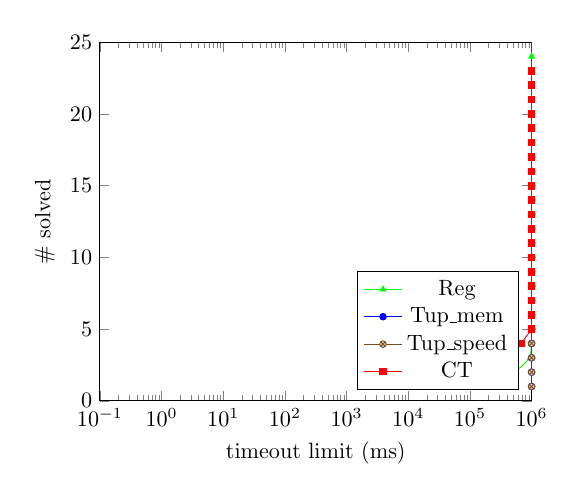
\begin{tikzpicture}[scale=0.8]
      \begin{axis}[
    xmode=log,
    ymin=0,ymax=25,
    xmin=0.1, xmax=1000000,
    every axis plot/.style={thin},
    xlabel={timeout limit (ms)},
    ylabel={\# solved},
    legend pos=south east
    % table/create on use/cumulative distribution/.style={
    %   create col/expr={\pgfmathaccuma + \thisrow{f(x)}}   
    % }
    ]
    \addplot 
    [mark=triangle*,
    mark size=1.5,
    mark options={solid},
    green] 
    coordinates {(362179.365, 1)
(542610.443, 2)
(956273.144, 3)
(1000000.188, 4)
(1000000.201, 5)
(1000000.201, 6)
(1000000.220, 7)
(1000000.266, 8)
(1000000.268, 9)
(1000000.291, 10)
(1000000.294, 11)
(1000000.295, 12)
(1000000.297, 13)
(1000000.329, 14)
(1000000.339, 15)
(1000000.376, 16)
(1000000.377, 17)
(1000000.409, 18)
(1000000.412, 19)
(1000000.463, 20)
(1000000.483, 21)
(1000000.641, 22)
(1000000.668, 23)
(1000000.801, 24)
(1029699.464, 25)};

    \addplot 
    [blue,
    mark=*,
    mark size=1.5,
    mark options={solid}]
    coordinates {(1000001.069, 1)
(1000001.150, 2)
(1000001.274, 3)
(1000001.277, 4)
(1000001.523, 5)
(1000002.056, 6)
(1000002.073, 7)
(1000002.311, 8)
(1000002.579, 9)
(1000002.756, 10)
(1000003.085, 11)
(1000004.834, 12)
(1000004.876, 13)
(1000005.836, 14)
(1000005.855, 15)
(1000006.115, 16)
(1000006.863, 17)
(1000007.924, 18)
(1000008.395, 19)
(1000008.443, 20)
(1000009.040, 21)
(1000013.352, 22)
(1000013.437, 23)
(1000013.463, 24)
(1022769.751, 25)};

    \addplot [brown!60!black,
    mark options={fill=brown!40},
    mark=otimes*,
    mark size=1.5]
    coordinates {(1000000.597, 1)
(1000000.598, 2)
(1000000.770, 3)
(1000000.849, 4)
(1000001.124, 5)
(1000001.175, 6)
(1000001.309, 7)
(1000001.317, 8)
(1000001.461, 9)
(1000001.753, 10)
(1000001.826, 11)
(1000002.114, 12)
(1000002.685, 13)
(1000003.527, 14)
(1000003.580, 15)
(1000003.656, 16)
(1000004.416, 17)
(1000005.342, 18)
(1000006.111, 19)
(1000006.504, 20)
(1000007.848, 21)
(1000009.651, 22)
(1000010.626, 23)
(1000011.794, 24)
(1000016.468, 25)};

    \addplot 
    [red,
    mark size=1.5,
    mark=square*]
    coordinates {(45570.744, 1)
(97963.633, 2)
(284803.058, 3)
(676940.142, 4)
(1000000.180, 5)
(1000000.233, 6)
(1000000.268, 7)
(1000000.271, 8)
(1000000.295, 9)
(1000000.309, 10)
(1000000.312, 11)
(1000000.324, 12)
(1000000.334, 13)
(1000000.347, 14)
(1000000.351, 15)
(1000000.363, 16)
(1000000.386, 17)
(1000000.400, 18)
(1000000.453, 19)
(1000000.503, 20)
(1000000.579, 21)
(1000000.609, 22)
(1000000.673, 23)
(1019921.469, 24)
(1040148.010, 25)};
    \legend{Reg,Tup\_mem,Tup\_speed,CT}
  \end{axis}

    \end{tikzpicture}
    \vfill
    \caption{\textbf{MDD 05}.}
    \vspace{\baselineskip}
  \end{minipage}\qquad
  \begin{minipage}[b][10cm][s]{0.45\textwidth}
    \centering
    \vfill
    \begin{tikzpicture}[scale=0.8]
      \begin{tikzpicture}[scale=1.0]
  \begin{axis}[
    xmode=log,
    ymin=0,ymax=9,
    xmin=0.1, xmax=1000000,
    every axis plot/.style={thin},
    xlabel={timeout limit (ms)},
    ylabel={\# solved},
    legend pos=south east
    % table/create on use/cumulative distribution/.style={
    %   create col/expr={\pgfmathaccuma + \thisrow{f(x)}}   
    % }
    ]
    \addplot 
    [mark=triangle*,
    mark size=1.5,
    mark options={solid},
    green] 
    coordinates {8143.453 1
28227.868 2
30184.398 3
39636.695 4
40458.753 5
56228.579 6
66820.027 7
79866.961 8
245383.866 9};

    \addplot 
    [blue,
    mark=*,
    mark size=1.5,
    mark options={solid}]
    coordinates {1000001.471 1
1000001.544 2
1000002.625 3
1000002.721 4
1000002.899 5
1000003.208 6
1000004.208 7
1000004.650 8
1000005.052 9};

    \addplot [brown!60!black,
    mark options={fill=brown!40},
    mark=otimes*,
    mark size=1.5]
    table {1000000.498 1
1000000.780 2
1000000.821 3
1000001.078 4
1000001.299 5
1000001.505 6
1000002.168 7
1000004.073 8
1000008.854 9};

    \addplot 
    [red,
    mark size=1.5,
    mark=square*]
    table {1000000.160 1
1000000.224 2
1000000.247 3
1000000.259 4
1000000.300 5
1000000.307 6
1000000.343 7
1000000.404 8
1000000.445 9};
    \legend{Reg,Tup\_mem,Tup\_speed,CT}
  \end{axis}
\end{tikzpicture}

    \end{tikzpicture}
    \vfill
    \caption{\textbf{MDD 07}.}
    \vspace{\baselineskip}
  \end{minipage}\qquad
  \begin{minipage}[b][10cm][s]{.45\textwidth}
    \centering
    \vfill
    \begin{tikzpicture}[scale=0.8]
      \begin{tikzpicture}[scale=1.0]
  \begin{axis}[
    xmode=log,
    ymin=0,ymax=18,
    xmin=0.1, xmax=1000000,
    every axis plot/.style={thin},
    xlabel={timeout limit (ms)},
    ylabel={\# solved},
    legend pos=south east
    % table/create on use/cumulative distribution/.style={
    %   create col/expr={\pgfmathaccuma + \thisrow{f(x)}}   
    % }
    ]
    \addplot 
    [mark=triangle*,
    mark size=1.5,
    mark options={solid},
    green] 
    coordinates {160.082 1
199.047 2
738.646 3
1073.574 4
1941.132 5
4192.527 6
160.082 1
199.047 2
738.646 3
1073.574 4
1941.132 5
4192.527 6
(160.082,1)
(199.047,2)
(738.646,3)
(1073.574,4)
(1941.132,5)
(4192.527,6)};

    \addplot 
    [blue,
    mark=*,
    mark size=1.5,
    mark options={solid}]
    coordinates {1000001.385 1
1015679.482 2
1016279.242 3
1016406.246 4
1031535.613 5
1048711.823 6
1000001.385 1
1015679.482 2
1016279.242 3
1016406.246 4
1031535.613 5
1048711.823 6
(1000001.385,1)
(1015679.482,2)
(1016279.242,3)
(1016406.246,4)
(1031535.613,5)
(1048711.823,6)};

    \addplot [brown!60!black,
    mark options={fill=brown!40},
    mark=otimes*,
    mark size=1.5]
    table {1000000.720 1
1000001.967 2
1000005.371 3
1005327.065 4
1007653.014 5
1014601.258 6
1000000.720 1
1000001.967 2
1000005.371 3
1005327.065 4
1007653.014 5
1014601.258 6
(1000000.720,1)
(1000001.967,2)
(1000005.371,3)
(1005327.065,4)
(1007653.014,5)
(1014601.258,6)};

    \addplot 
    [red,
    mark size=1.5,
    mark=square*]
    table {1000000.477 1
1000881.615 2
1008283.620 3
1017720.801 4
1023341.972 5
1037219.927 6
1000000.477 1
1000881.615 2
1008283.620 3
1017720.801 4
1023341.972 5
1037219.927 6
(1000000.477,1)
(1000881.615,2)
(1008283.620,3)
(1017720.801,4)
(1023341.972,5)
(1037219.927,6)};
    \legend{Reg,Tup\_mem,Tup\_speed,CT}
  \end{axis}
\end{tikzpicture}

    \end{tikzpicture}
    \vfill
    \caption{\textbf{MDD 09}.}
    \vspace{\baselineskip}
  \end{minipage}\qquad
\end{figure}

\newpage

\begin{figure}
  \begin{minipage}[b][10cm][s]{0.45\textwidth}
    \centering
    \vfill
    \begin{tikzpicture}[scale=0.8]
      \begin{tikzpicture}[scale=1.0]
  \begin{axis}[
    xmode=log,
    ymin=0,ymax=314,
    xmin=0.1, xmax=1000000,
    every axis plot/.style={thin},
    xlabel={timeout limit (ms)},
    ylabel={\# solved},
    legend pos=south east
    % table/create on use/cumulative distribution/.style={
    %   create col/expr={\pgfmathaccuma + \thisrow{f(x)}}   
    % }
    ]
    \addplot 
    [mark=triangle*,
    mark size=1.5,
    mark options={solid},
    green] 
    table {./instances/kakuroext_easy/reg.data};

    \addplot 
    [blue,
    mark=*,
    mark size=1.5,
    mark options={solid}]
    table {./instances/kakuroext_easy/tup_mem.data};

    \addplot [brown!60!black,
    mark options={fill=brown!40},
    mark=otimes*,
    mark size=1.5]
    table {./instances/kakuroext_easy/tup_speed.data};

    \addplot 
    [red,
    mark size=1.5,
    mark=square*]
    table {./instances/kakuroext_easy/ct.data};
    \legend{Reg,Tup\_mem,Tup\_speed,CT}
  \end{axis}
\end{tikzpicture}

    \end{tikzpicture}
    \vfill
    \caption{\textbf{Kakuro easy}.}
    \vspace{\baselineskip}
  \end{minipage}\qquad



  \begin{minipage}[b][10cm][s]{0.45\textwidth}
    \centering
    \vfill
    \begin{tikzpicture}[scale=0.8]
      \begin{axis}[
    xmode=log,
    ymin=0,ymax=163,
    xmin=0.1, xmax=1000000,
    every axis plot/.style={thin},
    xlabel={timeout limit (ms)},
    ylabel={\# solved},
    legend pos=south east
    % table/create on use/cumulative distribution/.style={
    %   create col/expr={\pgfmathaccuma + \thisrow{f(x)}}   
    % }
    ]
    \addplot 
    [mark=triangle*,
    mark size=1.5,
    mark options={solid},
    green] 
    coordinates {(0.292, 1)
(0.366, 2)
(0.373, 3)
(0.375, 4)
(0.377, 5)
(0.388, 6)
(0.389, 7)
(0.390, 8)
(0.395, 9)
(0.395, 10)
(0.397, 11)
(0.398, 12)
(0.405, 13)
(0.406, 14)
(0.406, 15)
(0.409, 16)
(0.411, 17)
(0.413, 18)
(0.416, 19)
(0.420, 20)
(0.429, 21)
(0.442, 22)
(0.446, 23)
(0.449, 24)
(0.450, 25)
(0.453, 26)
(0.454, 27)
(0.457, 28)
(0.461, 29)
(0.462, 30)
(0.462, 31)
(0.465, 32)
(0.475, 33)
(0.479, 34)
(0.483, 35)
(0.498, 36)
(0.518, 37)
(0.526, 38)
(0.532, 39)
(0.533, 40)
(0.569, 41)
(0.606, 42)
(0.615, 43)
(0.619, 44)
(0.620, 45)
(0.627, 46)
(0.628, 47)
(0.639, 48)
(0.647, 49)
(0.652, 50)
(0.655, 51)
(0.655, 52)
(0.660, 53)
(0.667, 54)
(0.670, 55)
(0.671, 56)
(0.672, 57)
(0.676, 58)
(0.678, 59)
(0.682, 60)
(0.690, 61)
(0.696, 62)
(0.697, 63)
(0.699, 64)
(0.705, 65)
(0.706, 66)
(0.714, 67)
(0.721, 68)
(0.724, 69)
(0.724, 70)
(0.725, 71)
(0.729, 72)
(0.729, 73)
(0.739, 74)
(0.740, 75)
(0.752, 76)
(0.755, 77)
(0.756, 78)
(0.762, 79)
(0.764, 80)
(0.765, 81)
(0.770, 82)
(0.773, 83)
(0.776, 84)
(0.778, 85)
(0.781, 86)
(0.782, 87)
(0.784, 88)
(0.791, 89)
(0.792, 90)
(0.792, 91)
(0.795, 92)
(0.798, 93)
(0.809, 94)
(0.811, 95)
(0.818, 96)
(0.840, 97)
(0.843, 98)
(0.850, 99)
(0.865, 100)
(0.875, 101)
(0.876, 102)
(0.879, 103)
(0.883, 104)
(0.919, 105)
(0.946, 106)
(0.956, 107)
(0.973, 108)
(0.982, 109)
(0.991, 110)
(0.993, 111)
(1.013, 112)
(1.028, 113)
(1.128, 114)
(1.220, 115)
(1.629, 116)
(1.937, 117)
(1.984, 118)
(2.002, 119)
(2.141, 120)
(2.188, 121)
(2.223, 122)
(2.373, 123)
(2.728, 124)
(6.575, 125)
(16.845, 126)
(16.868, 127)
(17.495, 128)
(20.180, 129)
(47.620, 130)
(55.482, 131)
(67.498, 132)
(67.776, 133)
(155.334, 134)
(156.640, 135)
(167.546, 136)
(172.809, 137)
(196.818, 138)
(204.653, 139)
(204.863, 140)
(217.964, 141)
(329.079, 142)
(389.985, 143)
(407.197, 144)
(523.926, 145)
(697.290, 146)
(887.001, 147)
(898.340, 148)
(1081.375, 149)
(1084.068, 150)
(1174.012, 151)
(1425.046, 152)
(1584.244, 153)
(1628.143, 154)
(1868.481, 155)
(2070.450, 156)
(2163.404, 157)
(2425.521, 158)
(2641.938, 159)
(7228.341, 160)
(7393.205, 161)
(7834.491, 162)
(13216.356, 163)};

    \addplot 
    [blue,
    mark=*,
    mark size=1.5,
    mark options={solid}]
    coordinates {(0.242, 1)
(0.303, 2)
(0.419, 3)
(0.438, 4)
(0.452, 5)
(0.458, 6)
(0.461, 7)
(0.465, 8)
(0.490, 9)
(0.493, 10)
(0.494, 11)
(0.494, 12)
(0.498, 13)
(0.503, 14)
(0.508, 15)
(0.516, 16)
(0.517, 17)
(0.538, 18)
(0.542, 19)
(0.551, 20)
(0.552, 21)
(0.565, 22)
(0.566, 23)
(0.586, 24)
(0.590, 25)
(0.612, 26)
(0.638, 27)
(0.643, 28)
(0.656, 29)
(0.657, 30)
(0.666, 31)
(0.670, 32)
(0.713, 33)
(0.729, 34)
(0.730, 35)
(0.740, 36)
(0.765, 37)
(0.789, 38)
(0.793, 39)
(0.822, 40)
(0.843, 41)
(0.848, 42)
(0.866, 43)
(0.878, 44)
(0.879, 45)
(0.881, 46)
(0.884, 47)
(0.891, 48)
(0.913, 49)
(0.941, 50)
(0.941, 51)
(0.942, 52)
(0.959, 53)
(0.984, 54)
(0.993, 55)
(0.998, 56)
(1.004, 57)
(1.007, 58)
(1.008, 59)
(1.015, 60)
(1.028, 61)
(1.060, 62)
(1.063, 63)
(1.078, 64)
(1.084, 65)
(1.105, 66)
(1.109, 67)
(1.132, 68)
(1.132, 69)
(1.139, 70)
(1.143, 71)
(1.192, 72)
(1.200, 73)
(1.223, 74)
(1.240, 75)
(1.245, 76)
(1.250, 77)
(1.268, 78)
(1.279, 79)
(1.343, 80)
(1.356, 81)
(1.369, 82)
(1.386, 83)
(1.438, 84)
(1.495, 85)
(1.561, 86)
(1.588, 87)
(1.599, 88)
(1.663, 89)
(1.671, 90)
(1.690, 91)
(1.839, 92)
(1.841, 93)
(1.864, 94)
(1.915, 95)
(1.972, 96)
(2.012, 97)
(2.023, 98)
(2.056, 99)
(2.079, 100)
(2.084, 101)
(2.117, 102)
(2.205, 103)
(2.237, 104)
(2.261, 105)
(2.308, 106)
(2.312, 107)
(2.341, 108)
(2.385, 109)
(2.398, 110)
(2.522, 111)
(2.534, 112)
(2.580, 113)
(2.639, 114)
(2.696, 115)
(2.891, 116)
(3.074, 117)
(3.110, 118)
(3.168, 119)
(3.201, 120)
(3.232, 121)
(3.395, 122)
(3.487, 123)
(3.559, 124)
(3.602, 125)
(3.912, 126)
(4.139, 127)
(4.489, 128)
(4.703, 129)
(5.104, 130)
(5.790, 131)
(6.335, 132)
(6.724, 133)
(7.557, 134)
(7.643, 135)
(8.503, 136)
(8.570, 137)
(12.437, 138)
(12.678, 139)
(14.789, 140)
(16.260, 141)
(27.598, 142)
(95.672, 143)
(110.298, 144)
(222.608, 145)
(285.892, 146)
(296.774, 147)
(305.273, 148)
(694.806, 149)
(787.648, 150)
(1192.779, 151)
(1330.528, 152)
(1607.857, 153)
(1690.387, 154)
(1785.734, 155)
(2183.007, 156)
(3619.265, 157)
(3725.830, 158)
(3776.058, 159)
(5648.925, 160)
(6436.441, 161)
(6572.117, 162)
(7516.565, 163)};

    \addplot [brown!60!black,
    mark options={fill=brown!40},
    mark=otimes*,
    mark size=1.5]
    table {(0.252, 1)
(0.272, 2)
(0.430, 3)
(0.456, 4)
(0.460, 5)
(0.462, 6)
(0.469, 7)
(0.476, 8)
(0.485, 9)
(0.488, 10)
(0.499, 11)
(0.505, 12)
(0.506, 13)
(0.513, 14)
(0.520, 15)
(0.521, 16)
(0.522, 17)
(0.524, 18)
(0.536, 19)
(0.552, 20)
(0.569, 21)
(0.583, 22)
(0.583, 23)
(0.587, 24)
(0.590, 25)
(0.616, 26)
(0.620, 27)
(0.624, 28)
(0.629, 29)
(0.629, 30)
(0.648, 31)
(0.649, 32)
(0.661, 33)
(0.709, 34)
(0.715, 35)
(0.728, 36)
(0.759, 37)
(0.766, 38)
(0.774, 39)
(0.777, 40)
(0.801, 41)
(0.824, 42)
(0.842, 43)
(0.848, 44)
(0.851, 45)
(0.853, 46)
(0.854, 47)
(0.861, 48)
(0.874, 49)
(0.883, 50)
(0.899, 51)
(0.911, 52)
(0.916, 53)
(0.939, 54)
(0.952, 55)
(0.953, 56)
(0.954, 57)
(0.962, 58)
(0.966, 59)
(0.969, 60)
(0.987, 61)
(0.994, 62)
(0.999, 63)
(0.999, 64)
(1.015, 65)
(1.018, 66)
(1.036, 67)
(1.039, 68)
(1.061, 69)
(1.076, 70)
(1.094, 71)
(1.124, 72)
(1.131, 73)
(1.134, 74)
(1.160, 75)
(1.162, 76)
(1.168, 77)
(1.227, 78)
(1.249, 79)
(1.260, 80)
(1.267, 81)
(1.278, 82)
(1.282, 83)
(1.340, 84)
(1.381, 85)
(1.383, 86)
(1.432, 87)
(1.519, 88)
(1.629, 89)
(1.652, 90)
(1.656, 91)
(1.709, 92)
(1.720, 93)
(1.733, 94)
(1.812, 95)
(1.888, 96)
(1.895, 97)
(1.909, 98)
(1.912, 99)
(1.938, 100)
(1.949, 101)
(2.023, 102)
(2.043, 103)
(2.192, 104)
(2.266, 105)
(2.280, 106)
(2.309, 107)
(2.323, 108)
(2.344, 109)
(2.382, 110)
(2.391, 111)
(2.467, 112)
(2.498, 113)
(2.514, 114)
(2.612, 115)
(2.669, 116)
(2.710, 117)
(2.878, 118)
(2.960, 119)
(3.013, 120)
(3.175, 121)
(3.208, 122)
(3.231, 123)
(3.253, 124)
(3.829, 125)
(3.924, 126)
(3.993, 127)
(4.225, 128)
(4.456, 129)
(5.082, 130)
(5.168, 131)
(5.772, 132)
(5.827, 133)
(6.316, 134)
(6.346, 135)
(7.043, 136)
(7.505, 137)
(8.291, 138)
(9.089, 139)
(11.923, 140)
(13.976, 141)
(18.191, 142)
(18.643, 143)
(20.647, 144)
(69.668, 145)
(74.795, 146)
(115.506, 147)
(148.505, 148)
(231.847, 149)
(295.125, 150)
(505.755, 151)
(870.117, 152)
(1404.011, 153)
(2104.344, 154)
(2292.593, 155)
(2592.405, 156)
(3540.481, 157)
(4131.337, 158)
(5016.836, 159)
(5458.729, 160)
(7273.350, 161)
(11071.498, 162)
(13744.251, 163)};

    \addplot 
    [red,
    mark size=1.5,
    mark=square*]
    table {(0.235, 1)
(0.264, 2)
(0.392, 3)
(0.398, 4)
(0.414, 5)
(0.419, 6)
(0.424, 7)
(0.431, 8)
(0.432, 9)
(0.434, 10)
(0.435, 11)
(0.437, 12)
(0.441, 13)
(0.442, 14)
(0.449, 15)
(0.450, 16)
(0.452, 17)
(0.454, 18)
(0.454, 19)
(0.457, 20)
(0.462, 21)
(0.463, 22)
(0.466, 23)
(0.472, 24)
(0.474, 25)
(0.481, 26)
(0.487, 27)
(0.493, 28)
(0.497, 29)
(0.497, 30)
(0.509, 31)
(0.509, 32)
(0.510, 33)
(0.520, 34)
(0.520, 35)
(0.528, 36)
(0.536, 37)
(0.557, 38)
(0.559, 39)
(0.570, 40)
(0.573, 41)
(0.582, 42)
(0.598, 43)
(0.608, 44)
(0.619, 45)
(0.671, 46)
(0.682, 47)
(0.707, 48)
(0.712, 49)
(0.713, 50)
(0.716, 51)
(0.716, 52)
(0.720, 53)
(0.721, 54)
(0.722, 55)
(0.725, 56)
(0.729, 57)
(0.744, 58)
(0.745, 59)
(0.749, 60)
(0.758, 61)
(0.764, 62)
(0.765, 63)
(0.767, 64)
(0.769, 65)
(0.770, 66)
(0.773, 67)
(0.775, 68)
(0.775, 69)
(0.778, 70)
(0.781, 71)
(0.785, 72)
(0.787, 73)
(0.789, 74)
(0.794, 75)
(0.803, 76)
(0.810, 77)
(0.816, 78)
(0.817, 79)
(0.819, 80)
(0.819, 81)
(0.820, 82)
(0.822, 83)
(0.832, 84)
(0.837, 85)
(0.860, 86)
(0.866, 87)
(0.867, 88)
(0.868, 89)
(0.873, 90)
(0.879, 91)
(0.901, 92)
(0.908, 93)
(0.916, 94)
(0.917, 95)
(0.919, 96)
(0.920, 97)
(0.922, 98)
(0.930, 99)
(0.942, 100)
(0.945, 101)
(0.946, 102)
(0.948, 103)
(0.960, 104)
(0.962, 105)
(0.965, 106)
(0.968, 107)
(0.969, 108)
(0.970, 109)
(0.971, 110)
(0.973, 111)
(0.974, 112)
(0.978, 113)
(0.978, 114)
(0.986, 115)
(0.990, 116)
(0.991, 117)
(0.999, 118)
(1.001, 119)
(1.007, 120)
(1.007, 121)
(1.015, 122)
(1.019, 123)
(1.021, 124)
(1.023, 125)
(1.027, 126)
(1.028, 127)
(1.030, 128)
(1.049, 129)
(1.053, 130)
(1.080, 131)
(1.119, 132)
(1.171, 133)
(1.208, 134)
(1.420, 135)
(2.298, 136)
(2.329, 137)
(2.419, 138)
(2.460, 139)
(2.514, 140)
(2.554, 141)
(2.577, 142)
(2.588, 143)
(2.747, 144)
(8.080, 145)
(27.708, 146)
(52.742, 147)
(67.644, 148)
(68.071, 149)
(149.965, 150)
(240.838, 151)
(694.991, 152)
(757.228, 153)
(832.413, 154)
(850.382, 155)
(1367.286, 156)
(2490.629, 157)
(3002.133, 158)
(3739.967, 159)
(4484.374, 160)
(6572.976, 161)
(7799.168, 162)
(12630.382, 163)};
    \legend{Reg,Tup\_mem,Tup\_speed,CT}
  \end{axis}

    \end{tikzpicture}
    \vfill
    \caption{\textbf{Kakuro Medium}.}
    \vspace{\baselineskip}
  \end{minipage}\qquad


  \begin{minipage}[b][10cm][s]{0.45\textwidth}
    \centering
    \vfill
    \begin{tikzpicture}[scale=0.8]
      \begin{tikzpicture}[scale=1.0]
  \begin{axis}[
    xmode=log,
    ymin=0,ymax=166,
    xmin=0.1, xmax=1000000,
    every axis plot/.style={thin},
    xlabel={timeout limit (ms)},
    ylabel={\# solved},
    legend pos=south east
    % table/create on use/cumulative distribution/.style={
    %   create col/expr={\pgfmathaccuma + \thisrow{f(x)}}   
    % }
    ]
    \addplot 
    [mark=triangle*,
    mark size=1.5,
    mark options={solid},
    green] 
    coordinates {0.142 1
0.228 2
0.338 3
0.352 4
0.352 5
0.355 6
0.356 7
0.359 8
0.368 9
0.371 10
0.374 11
0.384 12
0.384 13
0.388 14
0.389 15
0.393 16
0.395 17
0.396 18
0.397 19
0.397 20
0.400 21
0.401 22
0.407 23
0.407 24
0.408 25
0.413 26
0.417 27
0.423 28
0.427 29
0.428 30
0.432 31
0.433 32
0.438 33
0.444 34
0.451 35
0.454 36
0.454 37
0.457 38
0.458 39
0.459 40
0.461 41
0.462 42
0.463 43
0.469 44
0.475 45
0.492 46
0.507 47
0.537 48
0.538 49
0.547 50
0.573 51
0.579 52
0.582 53
0.590 54
0.590 55
0.601 56
0.603 57
0.610 58
0.619 59
0.619 60
0.619 61
0.623 62
0.632 63
0.637 64
0.639 65
0.642 66
0.646 67
0.646 68
0.648 69
0.649 70
0.658 71
0.658 72
0.661 73
0.662 74
0.665 75
0.667 76
0.674 77
0.676 78
0.677 79
0.680 80
0.682 81
0.684 82
0.685 83
0.695 84
0.702 85
0.704 86
0.706 87
0.707 88
0.711 89
0.711 90
0.712 91
0.716 92
0.716 93
0.717 94
0.720 95
0.722 96
0.722 97
0.725 98
0.726 99
0.729 100
0.729 101
0.733 102
0.734 103
0.743 104
0.758 105
0.758 106
0.762 107
0.771 108
0.772 109
0.776 110
0.778 111
0.779 112
0.788 113
0.793 114
0.801 115
0.818 116
0.822 117
0.827 118
0.829 119
0.830 120
0.833 121
0.838 122
0.853 123
0.854 124
0.871 125
0.887 126
0.914 127
0.917 128
0.921 129
0.930 130
0.935 131
1.002 132
1.025 133
1.026 134
1.029 135
1.136 136
1.163 137
1.182 138
1.259 139
1.287 140
1.419 141
1.468 142
1.555 143
1.691 144
2.007 145
2.187 146
4.778 147
28.309 148
57.741 149
89.280 150
207.765 151
226.921 152
341.161 153
376.096 154
381.080 155
393.442 156
401.976 157
493.187 158
622.427 159
683.805 160
940.071 161
992.845 162
1317.381 163
1449.577 164
1601.091 165
2061.896 166};

    \addplot 
    [blue,
    mark=*,
    mark size=1.5,
    mark options={solid}]
    coordinates {0.178 1
0.355 2
0.448 3
0.450 4
0.452 5
0.459 6
0.460 7
0.468 8
0.468 9
0.475 10
0.476 11
0.482 12
0.497 13
0.502 14
0.507 15
0.508 16
0.510 17
0.511 18
0.516 19
0.528 20
0.539 21
0.551 22
0.556 23
0.556 24
0.557 25
0.581 26
0.584 27
0.592 28
0.598 29
0.598 30
0.606 31
0.611 32
0.612 33
0.617 34
0.623 35
0.629 36
0.641 37
0.643 38
0.653 39
0.667 40
0.670 41
0.682 42
0.690 43
0.706 44
0.718 45
0.719 46
0.737 47
0.776 48
0.784 49
0.795 50
0.816 51
0.831 52
0.837 53
0.845 54
0.864 55
0.864 56
0.867 57
0.876 58
0.879 59
0.880 60
0.896 61
0.900 62
0.902 63
0.903 64
0.904 65
0.910 66
0.915 67
0.923 68
0.932 69
0.971 70
1.005 71
1.021 72
1.031 73
1.045 74
1.058 75
1.061 76
1.069 77
1.069 78
1.070 79
1.080 80
1.087 81
1.104 82
1.107 83
1.122 84
1.127 85
1.134 86
1.139 87
1.155 88
1.169 89
1.173 90
1.176 91
1.180 92
1.197 93
1.247 94
1.248 95
1.251 96
1.256 97
1.265 98
1.270 99
1.275 100
1.284 101
1.294 102
1.356 103
1.407 104
1.408 105
1.412 106
1.511 107
1.562 108
1.667 109
1.686 110
1.690 111
1.695 112
1.697 113
1.723 114
1.726 115
1.727 116
1.745 117
1.750 118
1.796 119
1.830 120
1.986 121
2.002 122
2.168 123
2.265 124
2.401 125
2.401 126
2.409 127
2.410 128
2.562 129
2.621 130
2.645 131
2.805 132
2.846 133
2.858 134
2.885 135
3.002 136
3.069 137
3.080 138
3.081 139
3.104 140
3.120 141
3.169 142
3.281 143
3.467 144
3.642 145
3.731 146
4.133 147
4.194 148
4.569 149
4.852 150
5.023 151
5.591 152
5.961 153
6.715 154
6.727 155
7.110 156
8.123 157
8.951 158
9.327 159
9.514 160
14.719 161
18.383 162
95.354 163
353.342 164
997.084 165
1711.327 166};

    \addplot [brown!60!black,
    mark options={fill=brown!40},
    mark=otimes*,
    mark size=1.5]
    table {0.219 1
0.355 2
0.423 3
0.438 4
0.440 5
0.447 6
0.447 7
0.458 8
0.461 9
0.517 10
0.520 11
0.538 12
0.541 13
0.552 14
0.559 15
0.583 16
0.584 17
0.590 18
0.592 19
0.599 20
0.604 21
0.613 22
0.615 23
0.622 24
0.622 25
0.625 26
0.627 27
0.638 28
0.639 29
0.646 30
0.649 31
0.650 32
0.660 33
0.662 34
0.670 35
0.677 36
0.680 37
0.682 38
0.683 39
0.691 40
0.695 41
0.697 42
0.698 43
0.698 44
0.705 45
0.726 46
0.731 47
0.764 48
0.770 49
0.773 50
0.785 51
0.806 52
0.821 53
0.847 54
0.862 55
0.876 56
0.880 57
0.885 58
0.885 59
0.909 60
0.912 61
0.919 62
0.921 63
0.934 64
0.938 65
0.942 66
0.950 67
0.952 68
0.972 69
0.977 70
0.990 71
0.995 72
1.003 73
1.005 74
1.019 75
1.020 76
1.038 77
1.047 78
1.061 79
1.069 80
1.081 81
1.085 82
1.104 83
1.109 84
1.112 85
1.113 86
1.130 87
1.147 88
1.167 89
1.172 90
1.176 91
1.202 92
1.215 93
1.218 94
1.245 95
1.245 96
1.261 97
1.269 98
1.287 99
1.314 100
1.357 101
1.363 102
1.372 103
1.385 104
1.396 105
1.471 106
1.472 107
1.491 108
1.491 109
1.512 110
1.530 111
1.550 112
1.614 113
1.625 114
1.683 115
1.689 116
1.727 117
1.777 118
1.862 119
1.924 120
1.998 121
2.006 122
2.073 123
2.115 124
2.139 125
2.152 126
2.243 127
2.261 128
2.278 129
2.300 130
2.344 131
2.387 132
2.486 133
2.648 134
2.687 135
2.770 136
3.049 137
3.129 138
3.247 139
3.413 140
3.475 141
3.569 142
3.602 143
3.636 144
4.001 145
4.749 146
5.018 147
5.090 148
5.662 149
6.295 150
6.530 151
6.810 152
7.075 153
7.459 154
7.640 155
7.933 156
9.060 157
15.969 158
29.772 159
87.360 160
102.644 161
171.184 162
201.411 163
404.233 164
413.149 165
528.641 166};

    \addplot 
    [red,
    mark size=1.5,
    mark=square*]
    table {0.230 1
0.334 2
0.357 3
0.374 4
0.383 5
0.384 6
0.389 7
0.409 8
0.412 9
0.413 10
0.413 11
0.431 12
0.433 13
0.433 14
0.434 15
0.438 16
0.442 17
0.442 18
0.447 19
0.448 20
0.450 21
0.457 22
0.459 23
0.459 24
0.474 25
0.475 26
0.478 27
0.480 28
0.485 29
0.494 30
0.502 31
0.505 32
0.506 33
0.508 34
0.513 35
0.516 36
0.516 37
0.516 38
0.518 39
0.520 40
0.521 41
0.528 42
0.540 43
0.550 44
0.557 45
0.560 46
0.562 47
0.568 48
0.581 49
0.587 50
0.589 51
0.591 52
0.607 53
0.622 54
0.636 55
0.647 56
0.651 57
0.659 58
0.661 59
0.674 60
0.677 61
0.695 62
0.696 63
0.696 64
0.698 65
0.702 66
0.704 67
0.707 68
0.710 69
0.714 70
0.718 71
0.721 72
0.724 73
0.731 74
0.732 75
0.734 76
0.736 77
0.737 78
0.739 79
0.749 80
0.751 81
0.754 82
0.757 83
0.759 84
0.760 85
0.761 86
0.765 87
0.769 88
0.769 89
0.771 90
0.772 91
0.776 92
0.780 93
0.786 94
0.793 95
0.795 96
0.797 97
0.799 98
0.801 99
0.803 100
0.803 101
0.804 102
0.819 103
0.823 104
0.826 105
0.829 106
0.832 107
0.835 108
0.836 109
0.841 110
0.846 111
0.856 112
0.859 113
0.864 114
0.866 115
0.869 116
0.874 117
0.880 118
0.880 119
0.887 120
0.894 121
0.899 122
0.906 123
0.907 124
0.911 125
0.911 126
0.923 127
0.932 128
0.943 129
0.954 130
0.957 131
0.958 132
0.963 133
0.965 134
0.980 135
0.981 136
0.984 137
0.985 138
0.999 139
1.005 140
1.011 141
1.020 142
1.029 143
1.032 144
1.034 145
1.052 146
1.053 147
1.059 148
1.068 149
1.089 150
1.129 151
1.249 152
1.257 153
1.436 154
1.519 155
2.328 156
2.545 157
2.586 158
2.621 159
2.642 160
2.702 161
30.592 162
31.460 163
74.644 164
435.027 165
1646.184 166};
    \legend{Reg,Tup\_mem,Tup\_speed,CT}
  \end{axis}
\end{tikzpicture}

    \end{tikzpicture}
    \vfill
    \caption{\textbf{Kakuro Hard}.}
    \vspace{\baselineskip}
  \end{minipage}\qquad
\end{figure}

\newpage

\begin{figure}
  \begin{minipage}[b][10cm][s]{0.45\textwidth}
    \centering
    \vfill
    \begin{tikzpicture}[scale=0.8]
      \begin{tikzpicture}[scale=1.0]
  \begin{axis}[
    xmode=log,
    ymin=0,ymax=15,
    xmin=0.1, xmax=1000000,
    every axis plot/.style={thin},
    xlabel={timeout limit (ms)},
    ylabel={\# solved},
    legend pos=south east
    % table/create on use/cumulative distribution/.style={
    %   create col/expr={\pgfmathaccuma + \thisrow{f(x)}}   
    % }
    ]
    \addplot 
    [mark=triangle*,
    mark size=1.5,
    mark options={solid},
    green] 
    coordinates {0.094 1
0.103 2
0.105 3
0.106 4
0.106 5
0.108 6
0.111 7
0.135 8
0.138 9
0.139 10
0.143 11
0.146 12
0.147 13
0.148 14
0.148 15};

    \addplot 
    [blue,
    mark=*,
    mark size=1.5,
    mark options={solid}]
    coordinates {507.741 1
677.384 2
953.532 3
1115.834 4
1165.768 5
1493.977 6
9207.006 7
9850.063 8
13526.871 9
16256.105 10
25103.486 11
31196.630 12
35646.183 13
114674.413 14
219336.179 15};

    \addplot [brown!60!black,
    mark options={fill=brown!40},
    mark=otimes*,
    mark size=1.5]
    table {672.485 1
814.969 2
1067.305 3
1600.629 4
1680.609 5
2014.622 6
13301.506 7
13571.938 8
18857.094 9
21725.057 10
34735.363 11
42587.462 12
51076.269 13
151568.002 14
299369.282 15};

    \addplot 
    [red,
    mark size=1.5,
    mark=square*]
    table {238.429 1
266.356 2
392.689 3
568.593 4
600.935 5
609.600 6
4557.050 7
4627.268 8
6237.444 9
7103.168 10
11748.022 11
13000.044 12
16831.605 13
52006.921 14
102348.407 15};
    \legend{Reg,Tup\_mem,Tup\_speed,CT}
  \end{axis}
\end{tikzpicture}

    \end{tikzpicture}
    \vfill
    \caption{\textbf{TSP 25}.}
    \vspace{\baselineskip}
  \end{minipage}\qquad
  \begin{minipage}[b][10cm][s]{0.45\textwidth}
    \centering
    \vfill
    \begin{tikzpicture}[scale=0.8]
      \begin{axis}[
    xmode=log,
    ymin=0,ymax=11,
    xmin=0.1, xmax=1000000,
    every axis plot/.style={thin},
    xlabel={timeout limit (ms)},
    ylabel={\# solved},
    legend pos=south east
    % table/create on use/cumulative distribution/.style={
    %   create col/expr={\pgfmathaccuma + \thisrow{f(x)}}   
    % }
    ]
    \addplot 
    [mark=triangle*,
    mark size=1.5,
    mark options={solid},
    green] 
    coordinates {(0.090, 1)
(0.107, 2)
(0.119, 3)
(0.130, 4)
(0.140, 5)
(0.141, 6)
(0.147, 7)
(0.152, 8)
(0.153, 9)
(0.253, 10)
(0.485, 11)};

    \addplot 
    [blue,
    mark=*,
    mark size=1.5,
    mark options={solid}]
    coordinates {(24.908, 1)
(101.909, 2)
(449.341, 3)
(508.375, 4)
(1078.967, 5)
(5188.104, 6)
(6236.225, 7)
(20893.960, 8)
(21757.559, 9)
(39390.620, 10)
(180113.690, 11)};

    \addplot [brown!60!black,
    mark options={fill=brown!40},
    mark=otimes*,
    mark size=1.5]
    table {(39.537, 1)
(155.194, 2)
(1168.300, 3)
(1237.365, 4)
(2342.007, 5)
(11124.448, 6)
(15197.002, 7)
(46149.630, 8)
(48536.889, 9)
(88441.633, 10)
(424148.536, 11)};

    \addplot 
    [red,
    mark size=1.5,
    mark=square*]
    table {(8.864, 1)
(25.120, 2)
(110.549, 3)
(119.770, 4)
(267.516, 5)
(743.323, 6)
(885.183, 7)
(4580.535, 8)
(5856.136, 9)
(11262.118, 10)
(43076.438, 11)};
    \legend{Reg,Tup\_mem,Tup\_speed,CT}
  \end{axis}

    \end{tikzpicture}
    \vfill
    \caption{\textbf{TSP Quat 20}.}
    \vspace{\baselineskip}
  \end{minipage}\qquad
\end{figure}

\newpage

\begin{figure}
  \begin{minipage}[b][10cm][s]{0.45\textwidth}
    \centering
    \vfill
    \begin{tikzpicture}[scale=0.8]
      \begin{tikzpicture}[scale=1.0]
  \begin{axis}[
    xmode=log,
    ymin=0,ymax=49,
    xmin=0.1, xmax=1000000,
    every axis plot/.style={thin},
    xlabel={timeout limit (ms)},
    ylabel={\# solved},
    legend pos=south east
    % table/create on use/cumulative distribution/.style={
    %   create col/expr={\pgfmathaccuma + \thisrow{f(x)}}   
    % }
    ]
    \addplot 
    [mark=triangle*,
    mark size=1.5,
    mark options={solid},
    green] 
    coordinates {0.090 1
0.092 2
0.094 3
0.094 4
0.094 5
0.095 6
0.095 7
0.095 8
0.096 9
0.096 10
0.096 11
0.097 12
0.098 13
0.098 14
0.098 15
0.098 16
0.098 17
0.099 18
0.099 19
0.099 20
0.099 21
0.099 22
0.099 23
0.099 24
0.099 25
0.100 26
0.101 27
0.102 28
0.125 29
0.127 30
0.127 31
0.128 32
0.129 33
0.130 34
0.130 35
0.130 36
0.131 37
0.133 38
0.133 39
0.133 40
0.134 41
0.136 42
0.137 43
0.137 44
0.139 45
0.141 46
0.142 47
0.147 48
0.150 49};

    \addplot 
    [blue,
    mark=*,
    mark size=1.5,
    mark options={solid}]
    coordinates {8.908 1
9.827 2
18.048 3
44.969 4
146.544 5
221.926 6
280.600 7
1000.181 8
15513.013 9
48631.945 10
59316.805 11
168805.480 12
415608.611 13
649574.201 14
907115.910 15
1000000.555 16
1000000.559 17
1000000.602 18
1000000.610 19
1000000.620 20
1000000.629 21
1000000.647 22
1000000.658 23
1000000.659 24
1000000.668 25
1000000.676 26
1000000.690 27
1000000.697 28
1000000.698 29
1000000.703 30
1000000.711 31
1000000.711 32
1000000.726 33
1000000.733 34
1000000.760 35
1000000.775 36
1000000.777 37
1000000.783 38
1000000.783 39
1000000.818 40
1000000.834 41
1000000.837 42
1000000.841 43
1000000.891 44
1000000.911 45
1000001.014 46
1000001.027 47
1000001.082 48
1000001.151 49};

    \addplot [brown!60!black,
    mark options={fill=brown!40},
    mark=otimes*,
    mark size=1.5]
    table {8.888 1
10.058 2
23.562 3
63.830 4
252.102 5
271.618 6
388.958 7
2008.685 8
22663.365 9
62548.705 10
103749.263 11
249342.517 12
557770.707 13
1000000.164 14
1000000.168 15
1000000.168 16
1000000.170 17
1000000.177 18
1000000.180 19
1000000.188 20
1000000.189 21
1000000.189 22
1000000.201 23
1000000.207 24
1000000.210 25
1000000.227 26
1000000.239 27
1000000.243 28
1000000.243 29
1000000.248 30
1000000.252 31
1000000.253 32
1000000.253 33
1000000.270 34
1000000.294 35
1000000.295 36
1000000.300 37
1000000.313 38
1000000.316 39
1000000.323 40
1000000.347 41
1000000.375 42
1000000.438 43
1000000.448 44
1000000.542 45
1000000.561 46
1000000.574 47
1000000.653 48
1000001.050 49};

    \addplot 
    [red,
    mark size=1.5,
    mark=square*]
    table {2.210 1
2.770 2
5.373 3
14.096 4
50.117 5
54.652 6
63.872 7
349.605 8
5835.733 9
13759.320 10
18438.411 11
61277.615 12
170563.334 13
328014.772 14
399164.764 15
1000000.135 16
1000000.135 17
1000000.145 18
1000000.147 19
1000000.151 20
1000000.152 21
1000000.154 22
1000000.156 23
1000000.156 24
1000000.160 25
1000000.164 26
1000000.168 27
1000000.178 28
1000000.206 29
1000000.211 30
1000000.214 31
1000000.217 32
1000000.222 33
1000000.223 34
1000000.226 35
1000000.232 36
1000000.233 37
1000000.243 38
1000000.246 39
1000000.253 40
1000000.290 41
1000000.300 42
1000000.320 43
1000000.326 44
1000000.412 45
1000000.588 46
1000000.601 47
1000000.734 48
1000000.739 49};
    \legend{Reg,Tup\_mem,Tup\_speed,CT}
  \end{axis}
\end{tikzpicture}

    \end{tikzpicture}
    \vfill
    \caption{\textbf{Mod Renault}.}
    \vspace{\baselineskip}
  \end{minipage}\qquad


  \begin{minipage}[b][10cm][s]{0.45\textwidth}
    \centering
    \vfill
    \begin{tikzpicture}[scale=0.8]
      \begin{tikzpicture}[scale=1.0]
  \begin{axis}[
    xmode=log,
    ymin=0,ymax=23,
    xmin=0.1, xmax=1000000,
    every axis plot/.style={thin},
    xlabel={timeout limit (ms)},
    ylabel={\# solved},
    legend pos=south east
    % table/create on use/cumulative distribution/.style={
    %   create col/expr={\pgfmathaccuma + \thisrow{f(x)}}   
    % }
    ]
    \addplot 
    [mark=triangle*,
    mark size=1.5,
    mark options={solid},
    green] 
    coordinates {2.061 1
2.222 2
2.343 3
13.332 4
14.268 5
15.104 6
15.889 7
109.031 8
110.541 9
117.356 10
151.134 11
595.639 12
881.991 13
962.946 14
1032.881 15
3571.243 16
8738.273 17
9422.763 18
10198.491 19
84255.437 20
94066.800 21
102163.535 22
113104.807 23};

    \addplot 
    [blue,
    mark=*,
    mark size=1.5,
    mark options={solid}]
    coordinates {13.308 1
25.778 2
109.155 3
196.144 4
504.491 5
871.518 6
3062.199 7
3317.779 8
4522.000 9
11223.335 10
24740.626 11
62843.392 12
89446.323 13
277131.253 14
849755.006 15
1000000.200 16
1000000.205 17
1000000.270 18
1000000.361 19
1000000.652 20
1000000.691 21
1000001.070 22
1019998.875 23};

    \addplot [brown!60!black,
    mark options={fill=brown!40},
    mark=otimes*,
    mark size=1.5]
    table {20.148 1
33.783 2
118.145 3
296.244 4
615.097 5
1441.338 6
3178.111 7
4428.906 8
5043.658 9
12901.393 10
24049.663 11
90810.902 12
94920.322 13
309000.856 14
837935.273 15
1000000.133 16
1000000.137 17
1000000.326 18
1000000.454 19
1000002.060 20
1000004.976 21
1015563.536 22
1024422.263 23};

    \addplot 
    [red,
    mark size=1.5,
    mark=square*]
    table {8.102 1
9.443 2
11.856 3
19.253 4
52.342 5
108.958 6
130.917 7
181.194 8
431.986 9
1622.253 10
2055.962 11
3407.771 12
12209.023 13
27037.945 14
35303.261 15
77776.335 16
542919.574 17
790588.466 18
1000000.137 19
1000000.155 20
1000000.217 21
1013506.447 22
1031033.344 23};
    \legend{Reg,Tup\_mem,Tup\_speed,CT}
  \end{axis}
\end{tikzpicture}

    \end{tikzpicture}
    \vfill
    \caption{\textbf{Pigeons Plus}.}
    \vspace{\baselineskip}
  \end{minipage}\qquad



  \begin{minipage}[b][10cm][s]{0.45\textwidth}
    \centering
    \vfill
    \begin{tikzpicture}[scale=0.8]
      \begin{tikzpicture}[scale=1.0]
  \begin{axis}[
    xmode=log,
    ymin=0,ymax=10,
    xmin=0.1, xmax=1000000,
    every axis plot/.style={thin},
    xlabel={timeout limit (ms)},
    ylabel={\# solved},
    legend pos=south east
    % table/create on use/cumulative distribution/.style={
    %   create col/expr={\pgfmathaccuma + \thisrow{f(x)}}   
    % }
    ]
    \addplot 
    [mark=triangle*,
    mark size=1.5,
    mark options={solid},
    green] 
    coordinates {4443.913 1
5243.411 2
5290.054 3
5342.111 4
7798.538 5
9971.022 6
11495.589 7
11519.750 8
11916.452 9
13290.969 10};

    \addplot 
    [blue,
    mark=*,
    mark size=1.5,
    mark options={solid}]
    coordinates {8089.756 1
12315.191 2
17701.661 3
17868.371 4
19222.605 5
28355.755 6
30397.314 7
39852.755 8
48158.681 9
50328.664 10};

    \addplot [brown!60!black,
    mark options={fill=brown!40},
    mark=otimes*,
    mark size=1.5]
    table {9514.798 1
12881.890 2
20258.447 3
21027.141 4
21394.179 5
33373.659 6
35052.564 7
47603.591 8
52750.032 9
55059.829 10};

    \addplot 
    [red,
    mark size=1.5,
    mark=square*]
    table {990.112 1
1076.772 2
1646.320 3
1877.322 4
2034.652 5
3153.218 6
3424.938 7
3497.979 8
4695.754 9
4914.964 10};
    \legend{Reg,Tup\_mem,Tup\_speed,CT}
  \end{axis}
\end{tikzpicture}

    \end{tikzpicture}
    \vfill
    \caption{\textbf{k5}.}
    \vspace{\baselineskip}
  \end{minipage}\qquad

  \begin{minipage}[b][10cm][s]{0.45\textwidth}
    \centering
    \vfill
    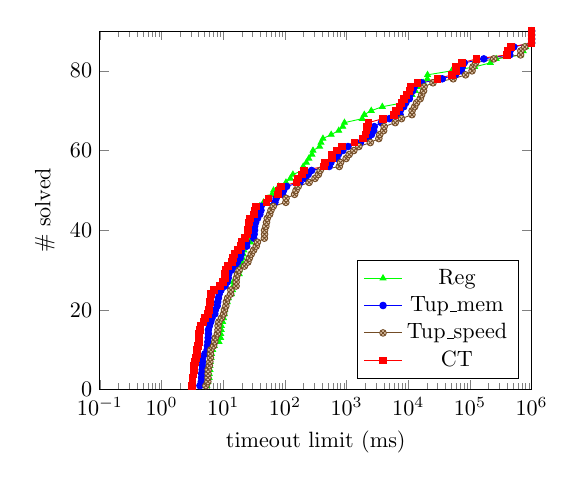
\begin{tikzpicture}[scale=0.8]
      \begin{axis}[
    xmode=log,
    ymin=0,ymax=90,
    xmin=0.1, xmax=1000000,
    every axis plot/.style={thin},
    xlabel={timeout limit (ms)},
    ylabel={\# solved},
    legend pos=south east
    % table/create on use/cumulative distribution/.style={
    %   create col/expr={\pgfmathaccuma + \thisrow{f(x)}}   
    % }
    ]
    \addplot 
    [mark=triangle*,
    mark size=1.5,
    mark options={solid},
    green] 
    coordinates {(5.389, 1)
(5.638, 2)
(5.908, 3)
(5.926, 4)
(6.086, 5)
(6.087, 6)
(6.166, 7)
(6.364, 8)
(6.469, 9)
(6.740, 10)
(7.148, 11)
(8.536, 12)
(9.080, 13)
(9.107, 14)
(9.303, 15)
(9.342, 16)
(9.805, 17)
(10.076, 18)
(10.428, 19)
(10.604, 20)
(10.907, 21)
(11.627, 22)
(12.123, 23)
(13.601, 24)
(14.151, 25)
(14.458, 26)
(14.490, 27)
(16.359, 28)
(18.190, 29)
(18.223, 30)
(18.413, 31)
(20.180, 32)
(20.506, 33)
(21.122, 34)
(21.643, 35)
(21.810, 36)
(27.563, 37)
(28.053, 38)
(28.274, 39)
(28.976, 40)
(30.018, 41)
(32.583, 42)
(32.814, 43)
(34.369, 44)
(38.523, 45)
(39.007, 46)
(44.977, 47)
(53.309, 48)
(61.875, 49)
(65.395, 50)
(79.428, 51)
(103.937, 52)
(122.565, 53)
(134.772, 54)
(193.149, 55)
(198.243, 56)
(223.375, 57)
(244.449, 58)
(274.390, 59)
(285.380, 60)
(365.560, 61)
(384.623, 62)
(413.842, 63)
(562.607, 64)
(746.251, 65)
(868.276, 66)
(924.223, 67)
(1793.623, 68)
(1937.966, 69)
(2509.726, 70)
(3797.584, 71)
(8373.485, 72)
(9593.391, 73)
(11531.366, 74)
(13031.885, 75)
(13941.016, 76)
(17694.770, 77)
(20392.242, 78)
(20545.405, 79)
(50620.318, 80)
(119540.736, 81)
(214612.883, 82)
(266484.425, 83)
(663627.605, 84)
(728667.872, 85)
(801665.108, 86)
(1000000.234, 87)
(1000000.344, 88)
(1000000.486, 89)
(1000000.515, 90)};

    \addplot 
    [blue,
    mark=*,
    mark size=1.5,
    mark options={solid}]
    coordinates {(4.188, 1)
(4.403, 2)
(4.451, 3)
(4.455, 4)
(4.562, 5)
(4.588, 6)
(4.619, 7)
(4.632, 8)
(5.046, 9)
(5.488, 10)
(5.538, 11)
(5.633, 12)
(5.705, 13)
(5.751, 14)
(5.756, 15)
(5.975, 16)
(6.278, 17)
(6.572, 18)
(7.295, 19)
(7.462, 20)
(7.979, 21)
(8.133, 22)
(8.358, 23)
(8.600, 24)
(9.209, 25)
(10.692, 26)
(11.548, 27)
(12.039, 28)
(12.248, 29)
(13.672, 30)
(15.880, 31)
(17.016, 32)
(18.711, 33)
(19.469, 34)
(19.729, 35)
(24.033, 36)
(24.051, 37)
(31.205, 38)
(31.687, 39)
(32.193, 40)
(32.329, 41)
(33.569, 42)
(35.982, 43)
(39.229, 44)
(40.895, 45)
(41.002, 46)
(68.982, 47)
(72.077, 48)
(91.486, 49)
(95.198, 50)
(106.573, 51)
(175.861, 52)
(214.260, 53)
(238.677, 54)
(271.193, 55)
(521.556, 56)
(557.425, 57)
(696.625, 58)
(735.011, 59)
(870.153, 60)
(1055.255, 61)
(1679.897, 62)
(2241.096, 63)
(2535.154, 64)
(2753.061, 65)
(2810.081, 66)
(3659.581, 67)
(4929.111, 68)
(7363.979, 69)
(7410.807, 70)
(8451.231, 71)
(9127.653, 72)
(10432.603, 73)
(10677.377, 74)
(11811.600, 75)
(12543.472, 76)
(16543.725, 77)
(35604.104, 78)
(58303.018, 79)
(72255.089, 80)
(75266.395, 81)
(80879.389, 82)
(167936.606, 83)
(442447.640, 84)
(447925.512, 85)
(514354.235, 86)
(1000001.142, 87)
(1000001.149, 88)
(1000001.277, 89)
(1000001.333, 90)};

    \addplot [brown!60!black,
    mark options={fill=brown!40},
    mark=otimes*,
    mark size=1.5]
    coordinates {(5.231, 1)
(5.629, 2)
(5.648, 3)
(5.663, 4)
(5.683, 5)
(5.943, 6)
(6.064, 7)
(6.179, 8)
(6.183, 9)
(6.295, 10)
(6.973, 11)
(7.284, 12)
(7.442, 13)
(8.037, 14)
(8.223, 15)
(8.238, 16)
(8.503, 17)
(9.384, 18)
(10.150, 19)
(10.464, 20)
(11.030, 21)
(11.224, 22)
(11.768, 23)
(13.192, 24)
(13.291, 25)
(16.148, 26)
(16.203, 27)
(16.372, 28)
(17.047, 29)
(18.087, 30)
(22.065, 31)
(25.084, 32)
(26.518, 33)
(28.470, 34)
(31.075, 35)
(34.278, 36)
(35.789, 37)
(46.424, 38)
(46.741, 39)
(46.749, 40)
(49.131, 41)
(50.337, 42)
(51.769, 43)
(56.622, 44)
(59.385, 45)
(64.673, 46)
(103.471, 47)
(104.380, 48)
(143.379, 49)
(151.391, 50)
(164.336, 51)
(246.920, 52)
(307.962, 53)
(349.129, 54)
(373.194, 55)
(761.064, 56)
(798.540, 57)
(984.391, 58)
(1100.413, 59)
(1311.163, 60)
(1581.664, 61)
(2426.014, 62)
(3330.803, 63)
(3451.164, 64)
(3985.165, 65)
(4060.894, 66)
(6149.120, 67)
(7773.303, 68)
(11478.659, 69)
(11534.975, 70)
(12707.939, 71)
(13658.601, 72)
(15631.173, 73)
(16480.122, 74)
(17709.931, 75)
(18042.131, 76)
(25195.852, 77)
(53588.555, 78)
(85036.871, 79)
(108170.261, 80)
(111741.798, 81)
(123479.329, 82)
(242924.139, 83)
(662412.696, 84)
(668282.082, 85)
(773006.352, 86)
(1000000.222, 87)
(1000000.350, 88)
(1000000.409, 89)
(1000001.208, 90)};

    \addplot 
    [red,
    mark size=1.5,
    mark=square*]
    coordinates {(3.077, 1)
(3.159, 2)
(3.165, 3)
(3.290, 4)
(3.360, 5)
(3.387, 6)
(3.499, 7)
(3.591, 8)
(3.773, 9)
(3.788, 10)
(3.878, 11)
(3.996, 12)
(3.998, 13)
(4.030, 14)
(4.235, 15)
(4.270, 16)
(4.806, 17)
(4.996, 18)
(5.677, 19)
(5.849, 20)
(5.952, 21)
(6.121, 22)
(6.164, 23)
(6.365, 24)
(7.079, 25)
(8.883, 26)
(9.951, 27)
(10.577, 28)
(10.722, 29)
(10.853, 30)
(11.910, 31)
(13.844, 32)
(14.533, 33)
(15.242, 34)
(17.301, 35)
(19.220, 36)
(19.624, 37)
(22.571, 38)
(24.789, 39)
(24.978, 40)
(25.692, 41)
(25.836, 42)
(27.326, 43)
(31.105, 44)
(32.150, 45)
(33.871, 46)
(50.022, 47)
(53.705, 48)
(77.777, 49)
(78.665, 50)
(86.000, 51)
(153.424, 52)
(163.326, 53)
(186.857, 54)
(205.347, 55)
(431.945, 56)
(447.896, 57)
(579.321, 58)
(582.538, 59)
(697.105, 60)
(845.847, 61)
(1342.019, 62)
(1841.060, 63)
(2032.310, 64)
(2086.544, 65)
(2136.864, 66)
(2259.967, 67)
(3859.192, 68)
(5928.297, 69)
(6294.023, 70)
(7189.658, 71)
(7718.920, 72)
(8552.721, 73)
(9394.659, 74)
(10400.047, 75)
(10914.835, 76)
(14065.923, 77)
(29727.731, 78)
(50913.845, 79)
(58766.196, 80)
(59010.473, 81)
(73352.608, 82)
(127355.852, 83)
(398786.693, 84)
(405416.242, 85)
(466149.784, 86)
(1000000.184, 87)
(1000000.216, 88)
(1000000.280, 89)
(1000000.721, 90)};
    \legend{Reg,Tup\_mem,Tup\_speed,CT}
  \end{axis}

    \end{tikzpicture}
    \vfill
    \caption{\textbf{Geom}.}
    \vspace{\baselineskip}
  \end{minipage}\qquad

\end{figure}

\newpage

\begin{figure}
  \begin{minipage}[b][10cm][s]{0.45\textwidth}
    \centering
    \vfill
    \begin{tikzpicture}[scale=0.8]
      \begin{axis}[
    xmode=log,
    ymin=0,ymax=13,
    xmin=0.1, xmax=1000000,
    every axis plot/.style={thin},
    xlabel={timeout limit (ms)},
    ylabel={\# solved},
    legend pos=south east
    % table/create on use/cumulative distribution/.style={
    %   create col/expr={\pgfmathaccuma + \thisrow{f(x)}}   
    % }
    ]
    \addplot 
    [mark=triangle*,
    mark size=1.5,
    mark options={solid},
    green] 
    coordinates {(25692.763, 1)
(52566.138, 2)
(108946.436, 3)
(221877.475, 4)
(464154.393, 5)
(959255.963, 6)
(1000000.112, 7)
(1000000.119, 8)
(1000000.125, 9)
(1000000.129, 10)
(1000000.202, 11)
(1000000.206, 12)
(1000000.220, 13)};

    \addplot 
    [blue,
    mark=*,
    mark size=1.5,
    mark options={solid}]
    coordinates {(24930.451, 1)
(51072.293, 2)
(104903.803, 3)
(218612.431, 4)
(452788.242, 5)
(938091.619, 6)
(1000000.148, 7)
(1000000.149, 8)
(1000000.179, 9)
(1000000.201, 10)
(1000000.213, 11)
(1000000.232, 12)
(1000000.236, 13)};

    \addplot [brown!60!black,
    mark options={fill=brown!40},
    mark=otimes*,
    mark size=1.5]
    table {(32168.167, 1)
(67198.233, 2)
(137576.561, 3)
(283937.740, 4)
(592360.368, 5)
(1000000.108, 6)
(1000000.110, 7)
(1000000.115, 8)
(1000000.116, 9)
(1000000.125, 10)
(1000000.180, 11)
(1000000.190, 12)
(1000000.202, 13)};

    \addplot 
    [red,
    mark size=1.5,
    mark=square*]
    table {(21084.624, 1)
(42987.264, 2)
(88183.028, 3)
(183554.060, 4)
(374851.071, 5)
(785860.510, 6)
(1000000.112, 7)
(1000000.115, 8)
(1000000.120, 9)
(1000000.183, 10)
(1000000.200, 11)
(1000000.202, 12)
(1061960.067, 13)};
    \legend{Reg,Tup\_mem,Tup\_speed,CT}
  \end{axis}

    \end{tikzpicture}
    \vfill
    \caption{\textbf{Dubois}.}
    \vspace{\baselineskip}
  \end{minipage}\qquad

\end{figure}

\newpage

\begin{figure}
  \begin{minipage}[b][10cm][s]{0.45\textwidth}
    \centering
    \vfill
    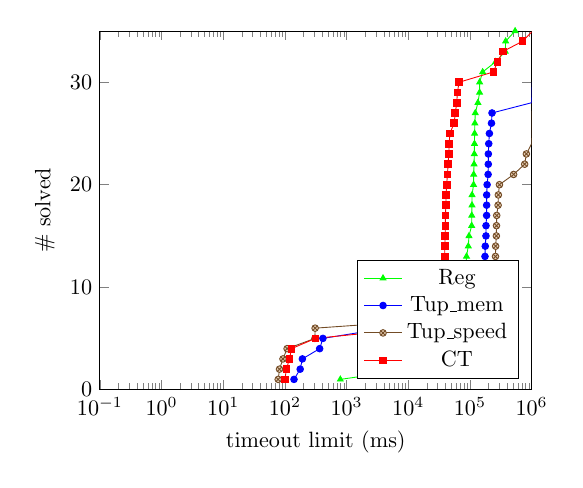
\begin{tikzpicture}[scale=0.8]
      \begin{axis}[
    xmode=log,
    ymin=0,ymax=35,
    xmin=0.1, xmax=1000000,
    every axis plot/.style={thin},
    xlabel={timeout limit (ms)},
    ylabel={\# solved},
    legend pos=south east
    % table/create on use/cumulative distribution/.style={
    %   create col/expr={\pgfmathaccuma + \thisrow{f(x)}}   
    % }
    ]
    \addplot 
    [mark=triangle*,
    mark size=1.5,
    mark options={solid},
    green] 
    coordinates {(791.560, 1)
(11472.600, 2)
(14766.696, 3)
(15745.163, 4)
(26862.099, 5)
(31778.084, 6)
(72448.015, 7)
(80752.168, 8)
(82923.009, 9)
(83683.963, 10)
(84465.445, 11)
(85764.561, 12)
(88032.555, 13)
(94011.079, 14)
(96560.156, 15)
(106648.859, 16)
(107056.591, 17)
(107933.416, 18)
(108210.305, 19)
(114497.218, 20)
(114966.358, 21)
(116658.706, 22)
(117735.741, 23)
(118508.245, 24)
(119006.430, 25)
(120178.594, 26)
(122120.270, 27)
(134711.654, 28)
(143405.319, 29)
(143582.718, 30)
(160788.320, 31)
(261709.502, 32)
(374501.791, 33)
(379347.315, 34)
(540015.740, 35)};

    \addplot 
    [blue,
    mark=*,
    mark size=1.5,
    mark options={solid}]
    coordinates {(140.425, 1)
(176.917, 2)
(192.112, 3)
(365.981, 4)
(413.133, 5)
(4403.296, 6)
(39876.347, 7)
(92306.099, 8)
(167189.458, 9)
(169366.958, 10)
(170556.481, 11)
(173851.037, 12)
(175430.330, 13)
(177265.457, 14)
(181905.169, 15)
(182312.517, 16)
(186399.578, 17)
(186652.401, 18)
(186832.299, 19)
(189971.439, 20)
(197152.408, 21)
(198415.969, 22)
(198894.284, 23)
(201831.845, 24)
(206792.806, 25)
(223634.515, 26)
(228125.105, 27)
(1001453.819, 28)
(1004586.749, 29)
(1020114.517, 30)
(1167495.643, 31)
(1316010.414, 32)
(1399844.041, 33)
(1422830.720, 34)
(1553624.496, 35)};

    \addplot [brown!60!black,
    mark options={fill=brown!40},
    mark=otimes*,
    mark size=1.5]
    coordinates {(77.848, 1)
(81.738, 2)
(93.013, 3)
(108.475, 4)
(306.721, 5)
(309.048, 6)
(71781.939, 7)
(119555.503, 8)
(232959.976, 9)
(235395.918, 10)
(237247.816, 11)
(247450.645, 12)
(259525.670, 13)
(261038.714, 14)
(268346.434, 15)
(269506.659, 16)
(271797.636, 17)
(286253.613, 18)
(288902.149, 19)
(300957.270, 20)
(510582.087, 21)
(771478.727, 22)
(822435.981, 23)
(1000367.652, 24)
(1005161.590, 25)
(1010019.345, 26)
(1010418.164, 27)
(1022093.039, 28)
(1029891.832, 29)
(1031150.393, 30)
(1034813.269, 31)
(1054519.771, 32)
(1073321.307, 33)
(1142503.375, 34)
(1301096.751, 35)};

    \addplot 
    [red,
    mark size=1.5,
    mark=square*]
    coordinates {(100.268, 1)
(105.476, 2)
(118.901, 3)
(127.592, 4)
(313.306, 5)
(13094.233, 6)
(19436.829, 7)
(34008.560, 8)
(35649.282, 9)
(36572.672, 10)
(36586.778, 11)
(38788.690, 12)
(39051.053, 13)
(39170.191, 14)
(39702.088, 15)
(39815.587, 16)
(40011.946, 17)
(40780.574, 18)
(40946.927, 19)
(41904.986, 20)
(43203.913, 21)
(44258.721, 22)
(45394.073, 23)
(46118.992, 24)
(47174.176, 25)
(55599.614, 26)
(57777.455, 27)
(61166.183, 28)
(62548.310, 29)
(66755.839, 30)
(239564.852, 31)
(281010.056, 32)
(343727.677, 33)
(713034.541, 34)
(1040781.786, 35)};
    \legend{Reg,Tup\_mem,Tup\_speed,CT}
  \end{axis}

    \end{tikzpicture}
    \vfill
    \caption{\textbf{BDD Large}.}
    \vspace{\baselineskip}
  \end{minipage}\qquad
\end{figure}
